\documentclass[b5paper, twoside, 11pt]{book}
\usepackage[utf8]{inputenc}
\usepackage[top=3cm,bottom=3cm,left=2cm,right=2cm,headsep=10pt]{geometry}
\usepackage{graphicx}
\usepackage{pdfpages} %[DW] used to import pdf pages
\usepackage{wrapfig}
\usepackage{enumitem} %[DW] used to get custome enumerate (in abstract list)
\usepackage{xcolor}
\usepackage{hyperref}

%%%%%%%%%%%%%%%%%%%%%%%%%%%%%%%%%%%%%%%
% [DW] customise footer / header  -start
\usepackage{fancyhdr}
\pagestyle{fancy}
\fancyhf{}
%may need to swap arguments depending on how pages fall - want page number at outer edge of each page
\fancyhead[LE,RO]{\thepage} %left-side of even pages, and right-side of odd
\fancyhead[RE,LO]{UKJEEL 2018}
%\fancyfoot[CE,CO]{\leftmark}
%\fancyfoot[LE,RO]{\thepage}
  
\renewcommand{\headrulewidth}{2pt}
%\renewcommand{\footrulewidth}{1pt}
% [DW] customise footer / header  -end
%%%%%%%%%%%%%%%%%%%%%%%%%%%%%%%%%%%%%%%


\renewcommand\thesection{\arabic{section}} %[DW] - cheap and cheerful way of getting section numbering w/out chapter number included

%\usepackage{hyperref} % [DW] Turns all instances of \ref and the t.o.c. into hyperlinks (must come just before \begin{document} - may be helpful if pdf version distributed
%\hypersetup{
%   colorlinks,
%    linkcolor={red!50!black},
%    citecolor={blue!50!black},
%    urlcolor={blue!80!black}
%}
\begin{document}
\frontmatter %[DW] Can only be used with 'book'
\renewcommand{\arraystretch}{1.25} % Increase the vertical padding about table cells

\thispagestyle{empty}
[Nice front cover showing Kyudai panorama and UKJEEL logos]

%\begin{titlepage}
\centering
	%\includegraphics[width=0.15\textwidth]{example-image-1x1}\par\vspace{1cm}
	{\scshape\LARGE\bfseries Proceedings of the 6th  UK-Japan \\
              Engineering Education League Workshop \par}
	\vspace{1cm}
	{\scshape\Large 3rd-5th September, 2018\\
               Nishijin Plaza, Fukuoka, Japan \par}
	\vspace{1.5cm}
	{\scshape\large Hosted by Kyushu University, Faculty of Engineering \par}
	\vspace{1.5cm}
	{\large\itshape \url{http://irose.kyushu-u.ac.jp/ukjeel} \\
                \url{https://www.facebook.com/UKJEEL/}  \par}
	\vfill
	 
% Bottom of the page
	{\scshape\large  Supported by Eight-University Engineering Association \\
          and 6U-HAPPIER \par }
\vspace{0.25cm}
{\scshape Proceedings Editors:  James J. Cannon  and Darren P. Wall \par }
\vspace{0.5cm}

\includegraphics[width=0.2\textwidth]{kyushu_log.jpg}\par\vspace{1cm}
\end{titlepage}

 

\section{Scientific Programme}

\begin{center}
{\bf \large Monday 3rd September}
\end{center}
\vspace*{3ex}
{\bf Morning session} (Venue: Nishijin Plaza, Fukuoka)\\
Chair: Assoc. Prof. James Cannon, Kyushu University

\vspace{1em}
\noindent\begin{tabular}{|l|l|}
    \hline
    08:30   & Doors open \\
    09:00   & Registration desk opens \\
    09:30   & Kyushu University welcoming remarks \\
            & \emph{Prof. Yoshio Hisaeda, Dean of Engineering, Kyushu University} \\
    09:45   & UKJEEL welcoming remarks \\
            & \emph{Prof. Roderick A Smith, Imperial College London, UKJEEL chair} \\
    10:00   & Keynote lecture: Challenge for unlimited molecular design aiming for high\\
            &  \hspace{7.5em} performance organic optoelectronic devices \\
            & \emph{Prof. Chihaya Adachi, Director of the Centre for Organic Photonics}\\
            & \emph{and Electronics Research, Kyushu University} \\
    10:40   & \emph{break} \\
    10:50   & Keynote lecture: Low dimensional materials for thermal application \\
            & \emph{Prof. Koji Takahashi, Dept. of Aeronautics and Astronautics,} \\
            & \emph{Kyushu University} \\
    11:30   & Lunch \& group photo \\
    \hline
\end{tabular}

\newpage
\vspace{-3em}
\noindent {\bf Afternoon session} (Venue: Nishijin Plaza, Fukuoka)\\
Chair: Prof. Yamada, Graduate School of Engineering, Kyushu University

\vspace{1em}
\noindent\begin{tabular}{|l|l|}
    \hline
    13:00   & Poster shotgun presentations \\
    13:30   & Poster session \\
    \emph{Faculty} & \\
    \hspace{1em}\emph{15:00} & Introduction by Prof. Kikuo Kishimoto, Tokyo Institute of \\
                             & Technology \\
    \hspace{1em}\emph{15:05} & Lecture: Assessment of Engineering Learning Outcomes Linking \\
                             & Abstract Program-level Competencies with Concrete/Course-level \\
                             & Learning Outcomes \\  
                             & \emph{Prof. Sakoto Fukahori,   UEII, Kyushu University} \\
    \hspace{1em}\emph{15:35} & Round-table discussion (finish 17:00) \\
    \emph{Students} & \\
    \hspace{1em}\emph{15:00} & Groupwork event (finish 18:00) \\
            & Chair: {\em Prof. Yasuyuki Takata, Kyushu University} \\
    17:15 \& 18:15   & Depart from Nishijin plaza \\
    19:00   & Dinner at Daruma-ya \\
    \hline
\end{tabular}

\newpage
\begin{center}
{\bf \large Tuesday 4th September}
\end{center}
\vspace*{3ex}
{\bf Morning session} (Venue: Nishijin Plaza, Fukuoka)\\
Chair: Prof. Sakoto Fukuhori,  The University Education Innovation Initiative, Kyushu University

\noindent\begin{tabular}{|l|l|}
    \hline
    09:55   & Announcements \\
    10:00   & Practical experience of implementing efficient Active Learning in the\\
            & classroom \\
            & \emph{Assoc. Prof. James Cannon, Dept. of Mechanical Engineering, Kyushu}\\
            & \emph{University} \\
    10:30   & The ins and outs of MOOC making \\
            & \emph{Prof. David Stewart, School of Engineering, Tokyo Institute of Technology} \\
    11:00   & Tokyo Tech’s edX MOOC production process, learning analytics, and\\
            & course utilization examples (on and off-campus) \\
            & \emph{Prof. Jeffery Cross, Dept. of Trandisciplinary Science and Engineering,} \\
            & \emph{Tokyo Institute of Technology} \\
    11:30   & Discussion \\
    12:00   & Lunch time and student discussion time \\

    \hline
\end{tabular}

\vspace*{3ex}
\noindent {\bf Afternoon session} (Venue: Nishijin Plaza, Fukuoka and Kyushu University, Ito Campus) \\
Chair: Prof. Yasuyuki Takata, Dept. of Mechanical Engineering, Kyushu University

\noindent\begin{tabular}{|l|l|}
    \hline
    13:30   & Student groupwork presentations \\
    14:30   & Closing remarks and announcements \\
    14:40   & Departure to Ito campus \\
    15:30   & Laboratory tours \\ % [locations to be mentioned here] \\
    \hspace{1em}$\mid$  & \\
    17:30   & \\
    18:00   & Conference Banquet at Suginoya \\
    \hline
\end{tabular}


\newpage
\begin{center}
{\bf \large Wednesday 5th September}
\end{center}
\vspace*{3ex}

\noindent\begin{tabular}{|l|l|}
    \hline
    09:00           & Departure from Tenjin (see maps)\\
    10:00 to 12:30  & Visit to Yanagawa including canal boat trip (weather permitting) \\
                    & and lunch\\
                    & \emph{or in case of inclement weather} \\
                    & Visit to Yame, including opportunities for experiencing Japanese \\
                    & paper and tea \\
    13:30 to 16:30  & Visit to Katana (sword) manufacturer \\
    17:30           & Arrival in Tenjin\\
    \hline
\end{tabular}


\tableofcontents


\mainmatter %[DW] Can only be used with 'book'
\section[Welcome messages]{Welcome message from the Dean of Engineering at Kyushu University, Prof. Yoshio Hisaeda}

\begin{wrapfigure}{r}{0.25\textwidth}
    \begin{center}
        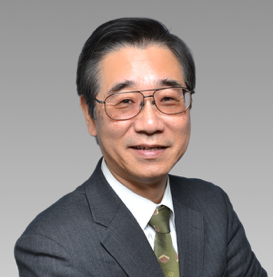
\includegraphics[width=0.23\textwidth]{hisaeda.png}
    \end{center}
\end{wrapfigure}

I am delighted to welcome you to the 6th UK-Japan Engineering Education League Workshop, held for the first time at Kyushu University. Given the long history of academic collaboration between the UK and Japan in fields of engineering education and research which extends back more than 150 years, this event represents a important continuation of cultural and scientific exchange for current and future generations of scientists, and we are proud to be the hosts of the 6th UKJEEL workshop.
 
The Faculty of Engineering in Kyushu University is the fourth oldest faculty among Japanese universities, and was founded as the College of Engineering of Kyushu Imperial University in 1911. Since that time, as one of the key faculties of the leading universities in Japan, the faculty has contributed to the development of engineering, technology and industry in Japan and worldwide, providing leading research and enhanced engineering education. This year is particularly momentous: the ceremony to celebrate completion of our new campus ``Ito Campus'' is being held this September.

I hope you all take this opportunity to build personal and professional connections between the Japanese and the UK scientific communities, and that your visit to Kyushu University and the wider Fukuoka region is an interesting and enjoyable one.

\vspace{1em}
\noindent Yoshio Hisaeda\\
Kyushu University\\
Dean of Engineering


\newpage
\section[Welcome messages]{Welcome message from the Chair of UKJEEL, Prof. Roderick A Smith}

\begin{wrapfigure}{r}{0.25\textwidth}
    \begin{center}
        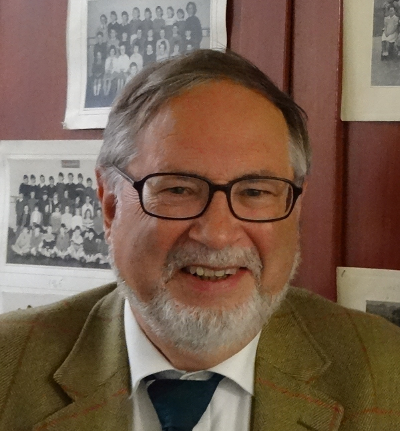
\includegraphics[width=0.23\textwidth]{smith.png}
    \end{center}
\end{wrapfigure}

I am delighted to welcome you to the 6th UK-Japan Engineering Education League Workshop, held for the first time at Kyushu University. Given the long history of academic collaboration between the UK and Japan in fields of engineering education and research which extends back more than 150 years, this event represents a important continuation of cultural and scientific exchange for current and future generations of scientists, and we are proud to be the hosts of the 6th UKJEEL workshop.
Welcome to Kyushu and its great university! 

Kyushu has been known throughout the history of Japan as a international gateway with particularly close links to Korea and China and, of course, the tiny trading island of Dejima in Nagasaki which maintained trading with the European nations even though the long period when Japan was officially closed.
 
In the next few days, during the 6th UK Japan Engineering Education League (UKJEEL) workshop, we are going to explore modern issues of materials engineering and the ways it might contribute to building a better earth in the future. To our young students here is an opportunity to become involved in the great issues which face us: Important because our future is in the hands of you and your colleagues all over the world, the engineers of the future. To our older faculty colleagues we will demonstrate that learning is a lifelong process and we discuss ideas to improve our teaching and enrich the learning experience we offer to our students. But we also have time to explore togther the delights of Kyushu, old and new. 

Kyushu University has a very strong international engineering presence. I am sure you will return home having fallen in love with this magical part of Japan: the interplay between sea and mountains, the wonderful food, the onsens and, of course, the warm and hospitable people.

Enjoy Kyushu and UKJEEL 2018!

\vspace{1em}
\noindent Roderick A Smith\\
Imperial College London\\
Chair UKJEEL

 % Smith, Hisaeda
\section{Conference organising committee}

\subsection*{Kyushu University}
\begin{tabular}{ll}
    Hiroshi Takamatsu & Professor, Dept. of Mechanical Engineering \\
    Masamichi Kohno & Professor, Dept. of Mechanical Engineering \\
    Yoshiko Miura   & Dept. of Chemical Systems and Engineering \\
    Kazuhiro Yasuda & Associate Professor, Dept. of Applied Quantum Physics and\\
                    & Nuclear Engineering \\
    James Cannon    & Associate Professor, Dept. of Mechanical Engineering \\
    John Chen       & Professor, Dept. of Mechanical Engineering \\
    Darren Wall     & Associate Professor,  Dept. of Aeronautics and Astronautics \\
    Teppei Yamada   & Associate Professor, Dept. of Chemical Engineering \\
    Chika Sonoda    & Technical Staff \\ 
                    & Dept. of Engineering International Education Support Centre \\
    Saori Maruno    & Technical Staff\\
                    & Dept. of Engineering International Education Support Centre \\
    Yumi Mizutani   & Technical Staff\\
                    & Dept. of Engineering International Education Support Centre \\
\end{tabular}

\subsection*{Tokyo Institute of Technology}

\begin{tabular}{ll}
    Jeffrey S. Cross & Professor, Tokyo Institute of Technology \\
    Daniel Berrar & Professor, Tokyo Institute of Technology \\
    Takeshi Kuroshima & Technical staff, Tokyo Institute of Technology \\
\end{tabular}

\section{List of Participants}
%[DW] May as well keep same format as organising committee ? 
%\subsection*{Faculty}
%\begin{tabular}{ll}
%Bilbo Baggins & Professor, Dept. of Mechanical Engineering, University of Middle Earth \\
%Bilbo Baggins & Professor, Dept. of Mechanical Engineering, University of Middle Earth 
%\end{tabular}

%\subsection*{Doctoral Students}
%\begin{tabular}{ll}
%Bilbo Baggins &  Dept. of Mechanical Engineering, University of Middle Earth \\
%Bilbo Baggins &   Dept. of Mechanical Engineering, University of Middle Earth 
%\end{tabular}

\begin{tabular}{lll}
Dr. Naoya Abe & Yasunori Aizawa & Mr. Rei Akahoshi \\
Mr. Seiji Azukizawa & Prof. Daniel Berrar & Prof. James Cannon \\
Prof. Qiang Chen & Mr. Xiaosheng Chen & Mr. Chitiphon Chuaicham \\
Dr. Yonghwan Cho & Prof. Jeffrey Cross & Ms. Yuka Fujiki \\
Mr. Georg Graninger & Prof. Yoshio Hisaeda & Mr. Sung Hwang \\
Prof. Shigekazu Ito & Prof. Nobuyuki Iwatsuki & Mr. Rikiya Kado \\
Dr. Tetsuya Kadonosono & Prof. Kuniyuki Kakushima & Prof. Kiyonobu Kasama \\
Ms. Naoto Kimura & Prof. Masamichi Kohno & Mr. Nattanai Kunanusont \\
Mr. Hikaru Kurasawa & Dr. Mu Li & Dr. Siyi Li \\
Mr. Jun Liu & Prof. Stephen Lyth & Mr. Khajeh Manafi \\
Dr. Stephane Matsushita & Prof. Tsuyoshi Michinobu & Prof. Yoshiko Miura \\
Ms. Nanoka Miyahara & Prof. Junko Morikawa & Mr. Yuya Murakami \\
Mr. Masamichi Murayama & Prof. Nobuo Nakada & Prof. Norihiro Nakai \\
Mr. Yutaka Nakano & Prof. Akinori Nishihara & Dr. Takumi Ohashi \\
Prof. Tatsuya Okubo & Prof. Yusuke Shimoyama & Dr. Nobuaki Shiraki \\
Mr. Dan Smith & Prof. Roderick A Smith & Prof. David Stewart \\
Dr. Yuko Suto & Prof. Atsushi Takahashi & Prof. Hiroshi Takamatsu \\
Mr. Kazuma Tanaka & Mr. Kazuki Tokumaru & Prof. Yuji Wada \\
Dr. Darren Wall & Prof. Wen Wang & Dr. Ian Watson \\
Dr. Elizabeth Webeck & Ms. Yuanhao Wu & Mr. Ji Xia \\
Prof. Kousuke Yakubo & Prof. Akira Yamada & Prof. Teppei Yamada \\
Prof. Kazuhiro Yasuda & Ms. Jaebong Yeon & \\
\end{tabular}

%Dr. Naoya Abe
%Yasunori Aizawa
%Mr. Rei Akahoshi
%Mr. Seiji Azukizawa
%Prof. Daniel Berrar
%Prof. James Cannon
%Prof. Qiang Chen
%Mr. Xiaosheng Chen
%Mr. Chitiphon Chuaicham
%Dr. Yonghwan Cho
%Prof. Jeffrey Cross
%Ms. Yuka Fujiki
%Mr. Georg Graninger
%Prof. Yoshio Hisaeda
%Mr. Sung Hwang
%Prof. Shigekazu Ito
%Prof. Nobuyuki Iwatsuki
%Mr. Rikiya Kado
%Dr. Tetsuya Kadonosono
%Prof. Kuniyuki Kakushima
%Prof. Kiyonobu Kasama
%Ms. Naoto Kimura
%Prof. Masamichi Kohno
%Mr. Nattanai Kunanusont
%Mr. Hikaru Kurasawa
%Dr. Mu Li
%Dr. Siyi Li
%Mr. Jun Liu
%Prof. Stephen Lyth
%Mr. Khajeh Manafi
%Dr. Stephane Matsushita
%Prof. Tsuyoshi Michinobu
%Prof. Yoshiko Miura
%Ms. Nanoka Miyahara
%Prof. Junko Morikawa
%Mr. Yuya Murakami
%Mr. Masamichi Murayama
%Prof. Nobuo Nakada
%Prof. Norihiro Nakai
%Mr. Yutaka Nakano
%Prof. Akinori Nishihara
%Dr. Takumi Ohashi
%Prof. Tatsuya Okubo
%Prof. Yusuke Shimoyama
%Dr. Nobuaki Shiraki
%Mr. Dan Smith
%Prof. Roderick A Smith
%Prof. David Stewart
%Dr. Yuko Suto
%Prof. Atsushi Takahashi
%Prof. Hiroshi Takamatsu
%Mr. Kazuma Tanaka
%Mr. Kazuki Tokumaru
%Prof. Yuji Wada
%Dr. Darren Wall
%Prof. Wen Wang
%Dr. Ian Watson
%Dr. Elizabeth Webeck
%Ms. Yuanhao Wu
%Mr. Ji Xia
%Prof. Kousuke Yakubo
%Prof. Akira Yamada
%Prof. Teppei Yamada
%Prof. Kazuhiro Yasuda
%Ms. Jaebong Yeon

 % List of participants
%\section{Kyushu University}
At regina gravi iamdudum saucia cura
vulnus alit venis et caeco carpitur igni.
multa viri virtus animo multusque recursat
gentis honos; haerent infixi pectore vultus
verbaque nec placidam membris dat cura quietem.       
postera Phoebea lustrabat lampade terras
umentemque Aurora polo dimoverat umbram,
cum sic unanimam adloquitur male sana sororem:
'Anna soror, quae me suspensam insomnia terrent!
quis novus hic nostris successit sedibus hospes,         
quem sese ore ferens, quam forti pectore et armis!
credo equidem, nec vana fides, genus esse deorum.
degeneres animos timor arguit. heu, quibus ille
iactatus fatis! quae bella exhausta canebat!
si mihi non animo fixum immotumque sederet              
ne cui me vinclo vellem sociare iugali,
postquam primus amor deceptam morte fefellit;
si non pertaesum thalami taedaeque fuisset,
huic uni forsan potui succumbere culpae.
Anna (fatebor enim) miseri post fata Sychaei           
coniugis et sparsos fraterna caede penatis
solus hic inflexit sensus animumque labantem
impulit. agnosco veteris vestigia flammae.
sed mihi vel tellus optem prius ima dehiscat
vel pater omnipotens adigat me fulmine ad umbras,         
pallentis umbras Erebo noctemque profundam,
ante, pudor, quam te violo aut tua iura resolvo.
ille meos, primus qui me sibi iunxit, amores
abstulit; ille habeat secum servetque sepulcro.'
sic effata sinum lacrimis implevit obortis.       
 % Information about Kyushu University
%\section{Tour Details}

\noindent\begin{tabular}{|l|l|}
    \hline
    09:00           & Departure from Tenjin\\
    10:00 to 12:30  & Visit to Yanagawa including canal boat trip (weather permitting) \\
                    & and lunch\\
                    & \emph{or in case of inclement weather} \\
                    & Visit to Yame, including opportunities for experiencing Japanese paper \\
                    & and tea \\
    13:30 to 16:30  & Visit to Katana (sword) manufacturer \\
    17:30           & Arrival in Tenjin\\
    \hline
\end{tabular}

\vspace{1em}
Please see maps page for departure map.
 % Tour information
%\pagenumbering{arabic}% resets `page` counter to 1
%\renewcommand*{\thepage}{A\arabic{page}}
%\appendix
\section{Abstracts}
\subsection*{List of Abstracts}
\begin{enumerate}[label=A\arabic*]
%\item B. Smith, Dept of Hard Sums, University of Central Nowhere, {\em Exact coherent state solutions in channel flow}

%\item A. Jones, Dept of Long Multiplication, Royal University of Somewhere, {\em New Exact Coherent States in Channel Flow}
\item R. Akahoshi,  Y.H. Cho, T. Nakamura  \& N. Mizutani, {\em Suspended Behavior of Clay on Mixed Sediment
under Regular Wave Action}

\item K. Aso, J. Maebe, T. Yamamoto \& S. Matsumura, {\em Precise measurement of lattice strain in gold
nanoparticles}

\item S. Azukizawa, H. Shinoda \&  F. Tsumori {\em Development of 4D Printing System
with Magnetic Anisotropy}

\item X. Chen, S. Suzuki,  M. Sakaguchi \& H. Inoue {\em Crystal plasticity analysis for temperature
dependent fatigue crack propagation in a single
crystal nickel-base superalloy}

\item Y. Fujiki \& K. Yakubo, {\em General framework to analyze long-range
degree correlations in complex networks}

\item G. Graninger, B.G. Falzon \& S. Kumar {\em Influence of filler size and melt processing routes
on the mechanical/thermal properties of cellulose
reinforced EVOH and NYLON composites}

\item N. Hirakawa, S. Fujikawa \& N. Kimizuka 1 {\em Fabrication of nanomembrane
with self-organized molecular channels
for preferential CO 2 separation}

\item S.H. Hwang, K. Kamataki, N. Itagaki, K. Koga, \& M. Shiratani {\em Effects of CH 4 Concentration on Size of
Carbon Nano-Particles Formed in Multi-hollow
Discharge Plasma}

\item R.Kado, G. Lelong, T. Kishi, G. Calas \& T. Yano, {\em Local structure of iron ions
in aluminosilicate glasses}

\item N. Kimura, N. Iwatsuki \& I. Ikeda, {\em Expansion of Kinematic Constraints in Linkage
Mechanism with New Joints}

\item     N. Kunanusont \& Y. Shimoyama, {\em Development of carbon porous electrode
for Li-O 2 /CO 2 battery using supercritical drying}

\item  H. Kurasawa, H. Yamashita \& Y. Aizawa, {\em Re-design and Synthesis of Yeast Chromosome}

\item M. Li \& M. Susa, {\em Thermal Conductivity Evaluation of Thermally
Grown FeO Scale on Steel}

\item J. Liu, C. Kaboglu, H. Liu, B.R.K. Blackman, A.J. Kinloch \& J.P. Dear, {\em
  High Speed Digital Image Correlation For Impact
Performance of Thermoplastic and Thermoset
Composites}

\item N. Miyahara, M. Shiratani \& N. Itagaki, {\em Photoluminescence of (ZnO) 0.92 (InN) 0.08 films
-Fabrication temperature dependence}

\item Y. Murakami \& Y. Shimoyama, {\em Continuous Production of Loposome
Using Supercritical-Fluid-Based Technique}

\item M. Murayama, H. Tsutsui \& S. Tsuji-Iio, {\em Neutron-induced Defect in First Wall of Nuclear
Fusion Reactor}

\item S. Nakano, K. Tanaka, H. Hara, L. Shi, D. Yamashita,
K. Kamataki, N. Itagaki, K. Koga \& Masaharu Shiratani, {\em Improvement of Si network order of a-Si:H thin
films by suppressing incorporation of
HOS molecules}

\item  Y. Ogawa, J. Yamabe, H. Matsunaga \& S. Matsuoka, {\em Hydrogen embrittlement resistance of a high-
strength copper-based alloy, CDA-C17200}

\item S.M.K. Pasha, H. Hazarika \& N. Yoshimoto, {\em Modeling Void Ratio Characteristics of Soil
Mixed with Recycled Tire Chips Using Artificial
Intelligence}

\item L. Siyi \& J. S. Cross, {\em  Modeling Void Ratio Characteristics of Soil
Mixed with Recycled Tire Chips Using Artificial
Intelligence}

\item D. Smith \& R. Douglas, {\em Fuzzy Rule-Based Energy Management Strategy
for a Parallel Mild-Hybrid Electric Bus}

\item K. Tokumaru \& F. Tsumori, {\em Micro Co-molding of Laminated Ceramic
Material by Imprinting Method}

\item Y. Wu, A. Mata \& W. Wang, {\em Molecular Co-assembly of a Peptide/protein 3D
Vessel for Bioengineering Applications}

\item   J. Xia, X. Xu, T. Omori \& R. Kainuma, {\em Entropy change during bcc/fcc martensitic
transformation in Fe-Mn-Al-Ni shape memory
alloy}

\item J. Yeon, M. Nakamoto \& T. Tanaka, {\em Joining of Metals using Super-Spread Wetting}


\end{enumerate}
\newpage
\pagenumbering{arabic}% resets `page` counter to 1
\renewcommand*{\thepage}{A\arabic{page}}
%\pageref{ab:smith}
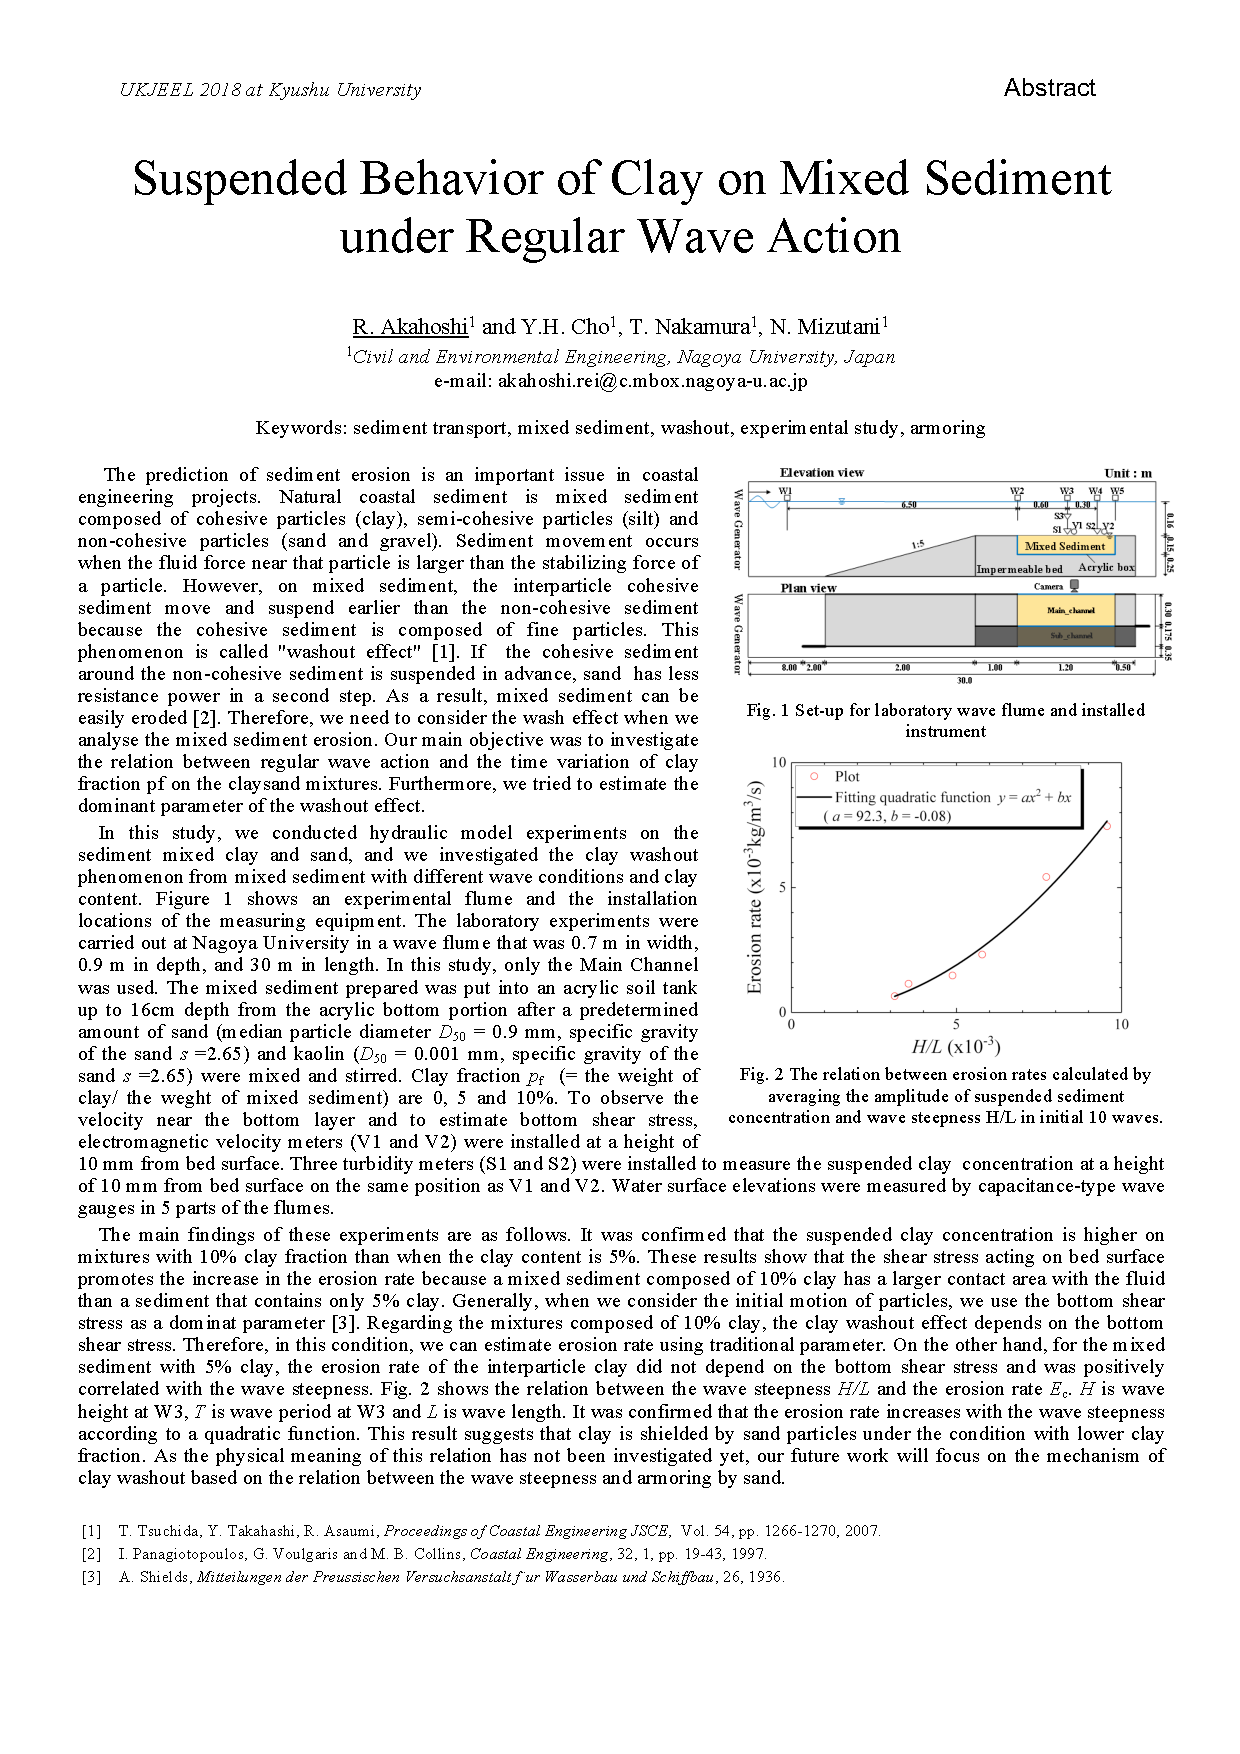
\includepdf[pagecommand={}, ]{abstracts/06-UKJEEL_AKAHOSHI-Rei.pdf}
%\pageref{ab:jones}
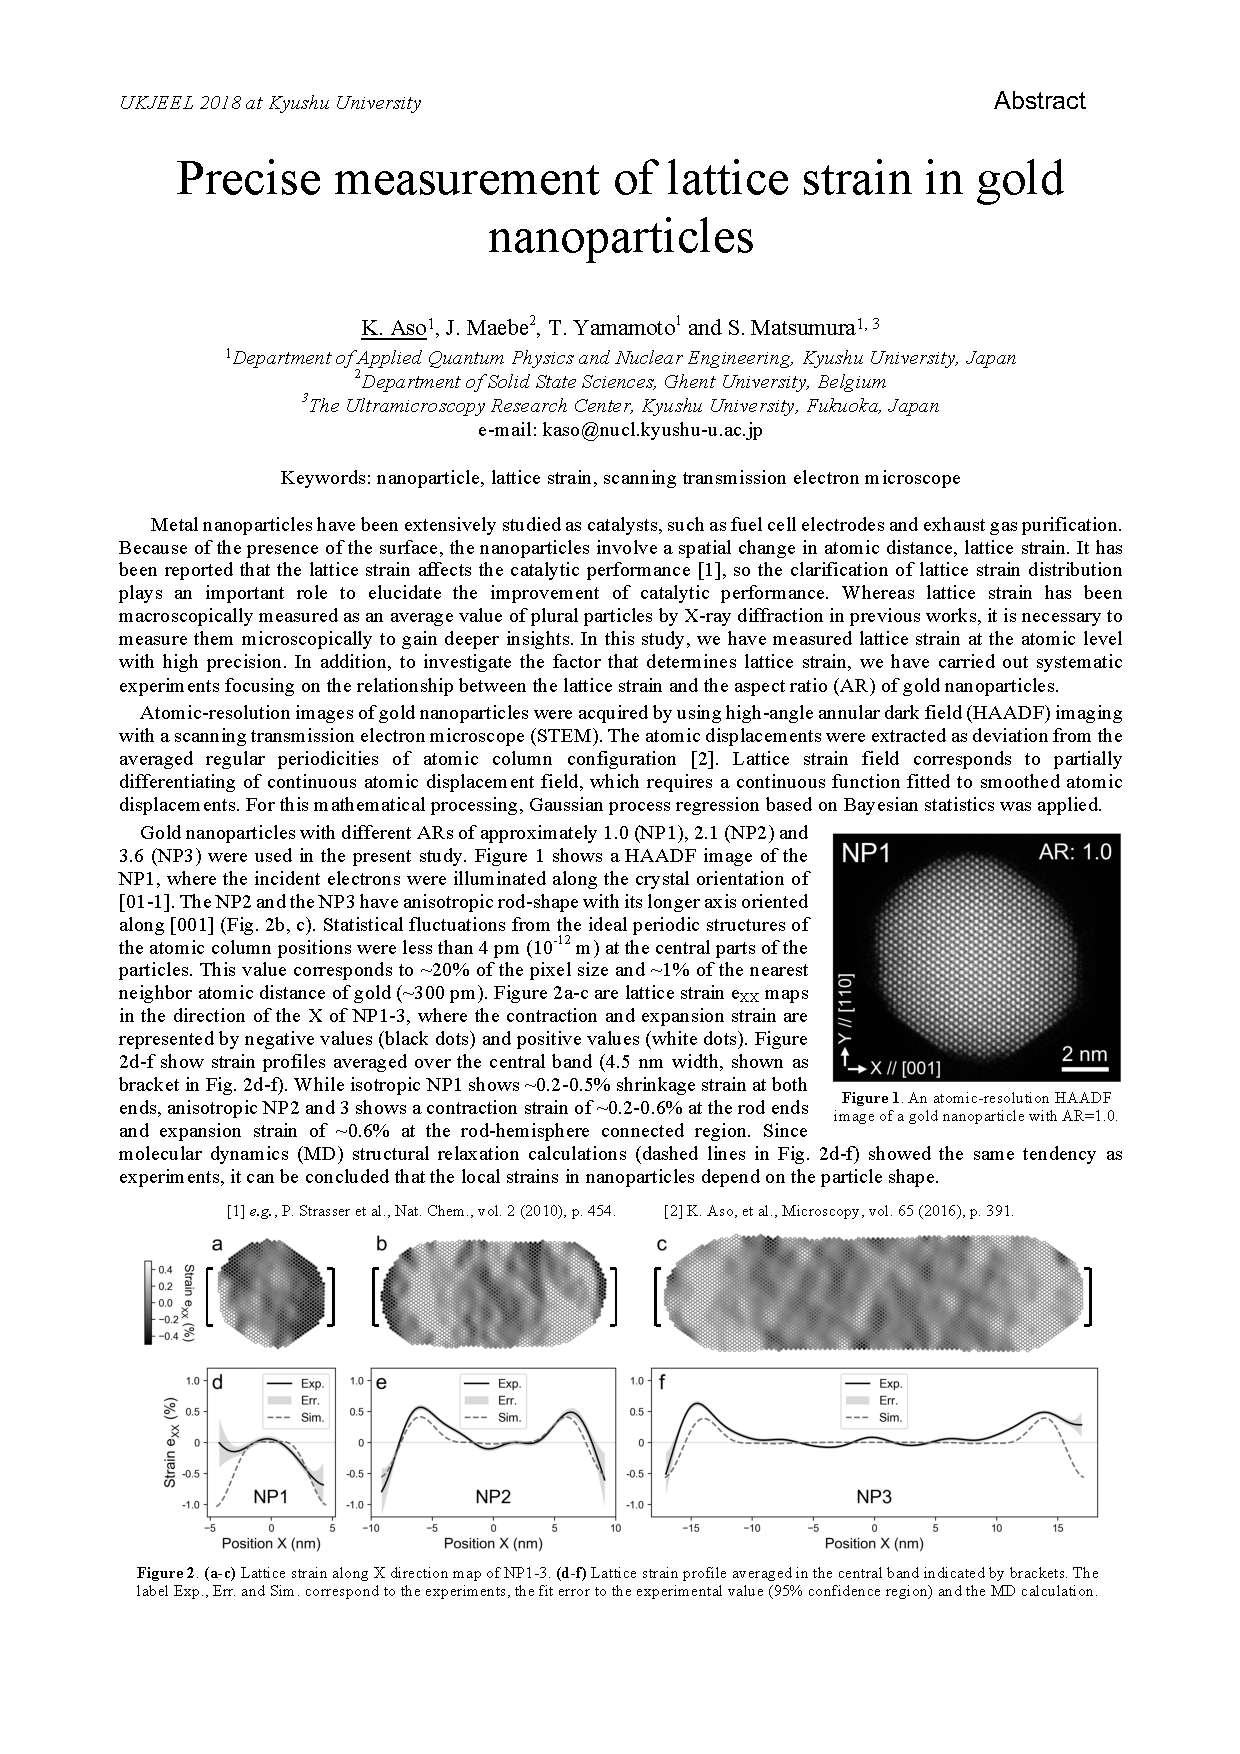
\includepdf[pagecommand={}]{abstracts/02-UKJEEL2018_aso.pdf}

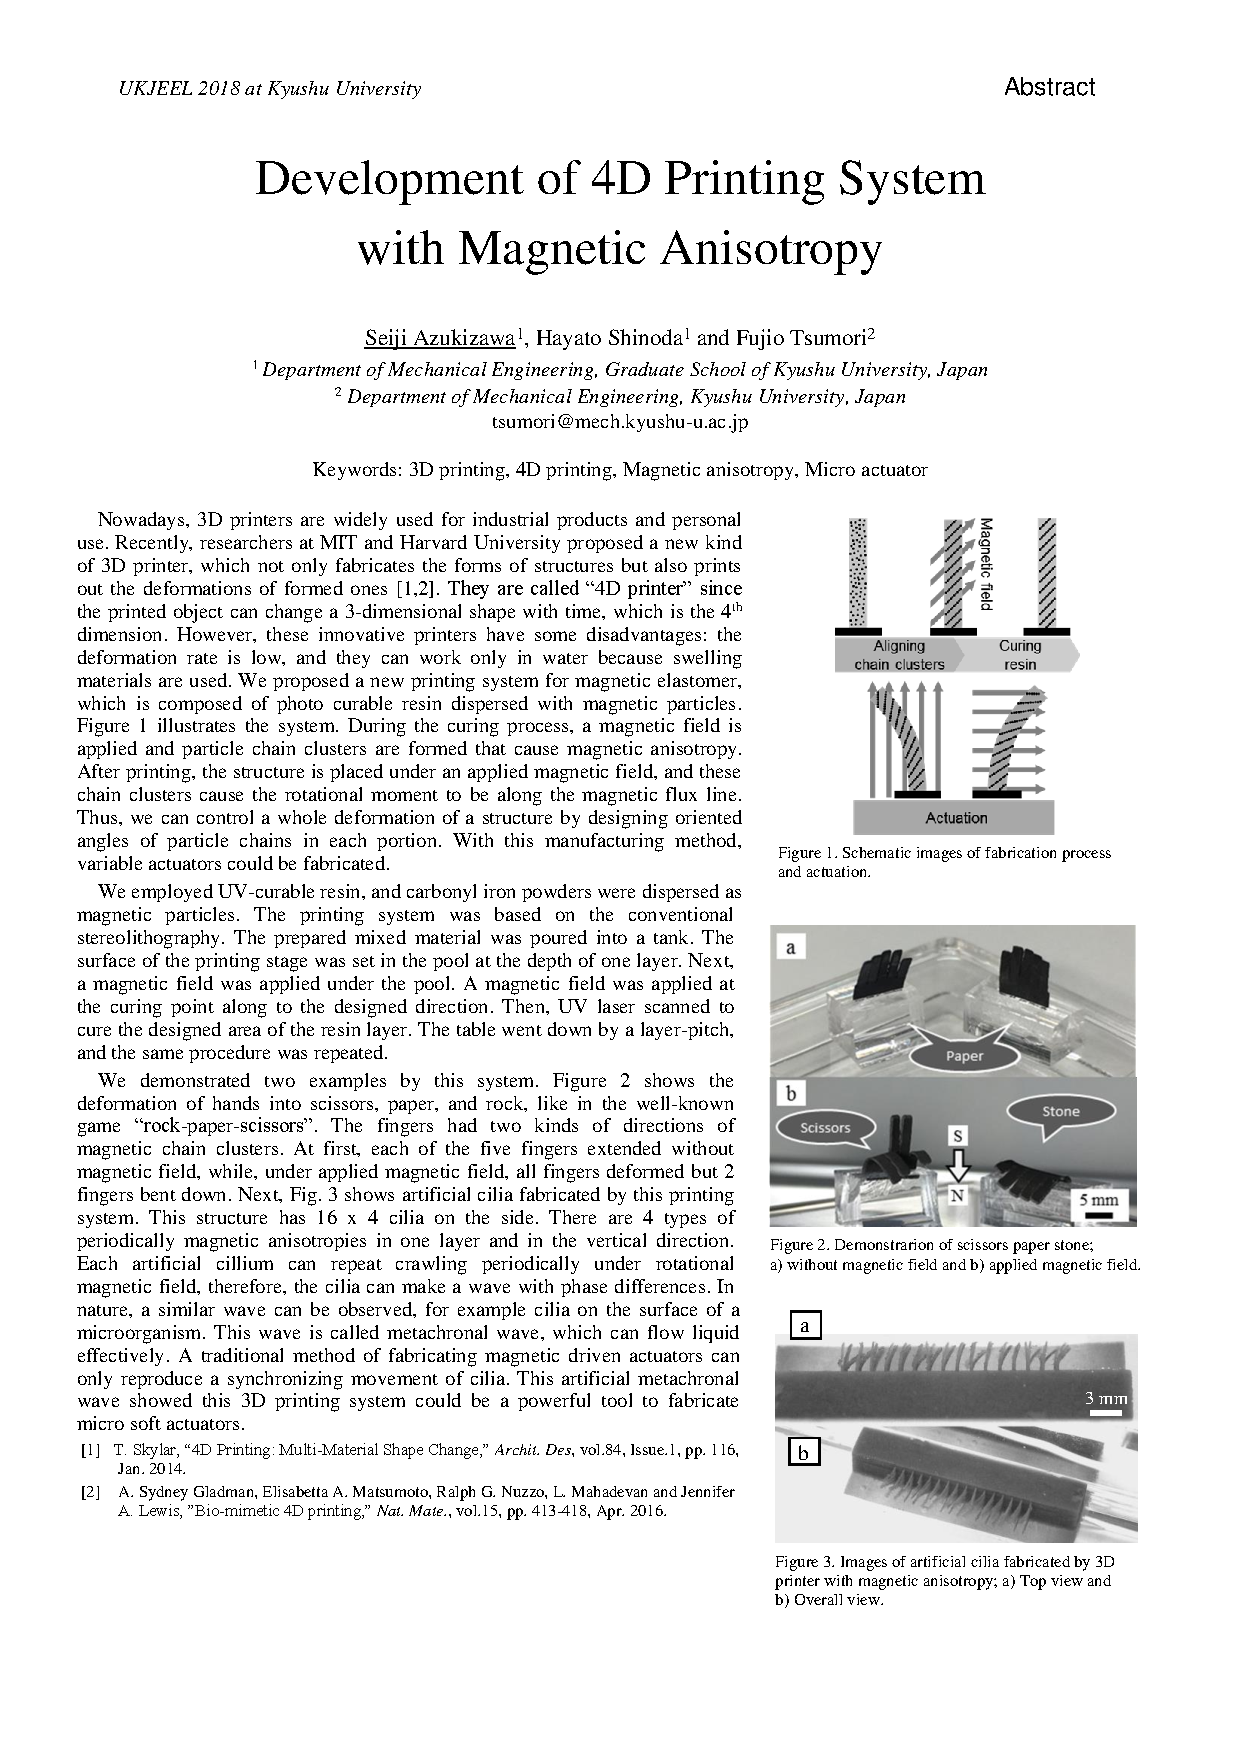
\includepdf[pagecommand={}]{abstracts/17-UKJEEL2018_Azukizawa.pdf}

 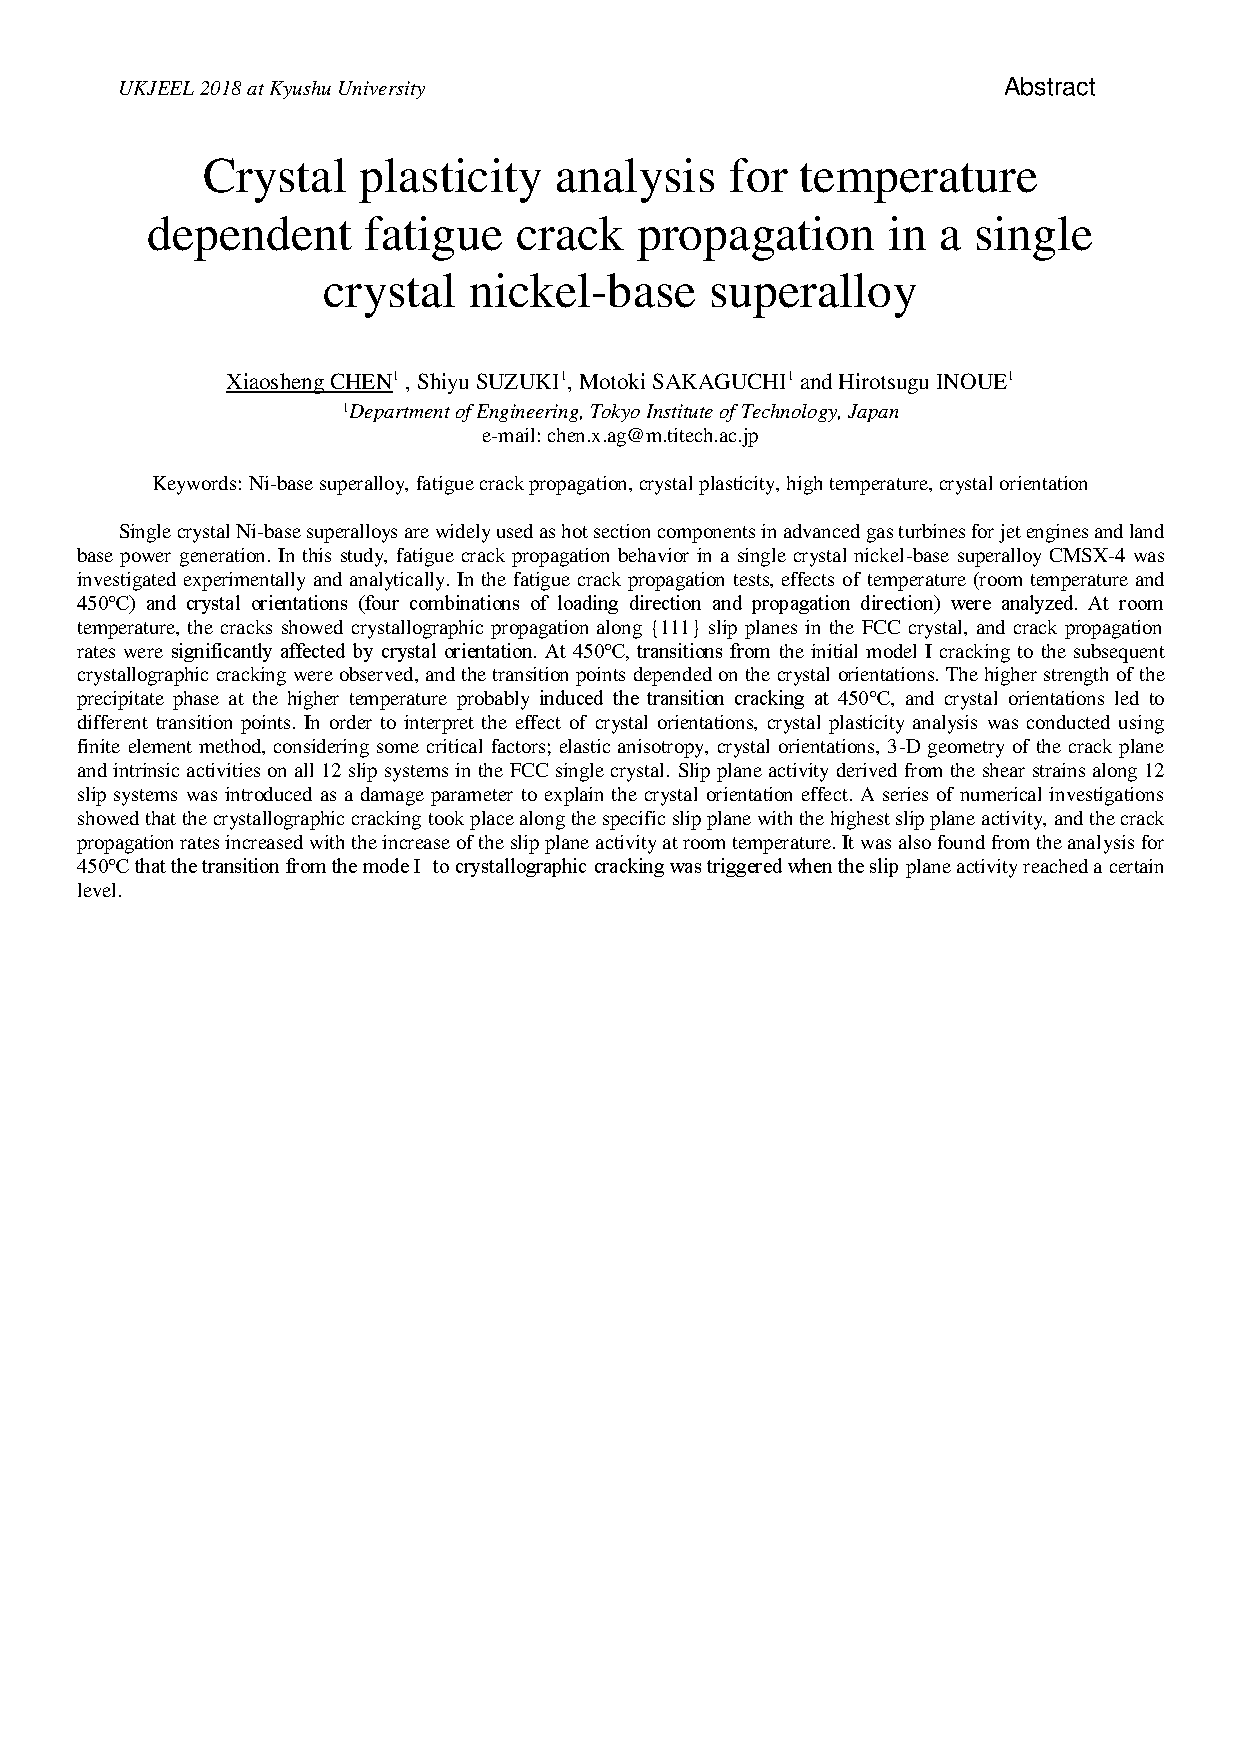
\includepdf[pagecommand={}]{abstracts/07-UKJEEL_CHEN-Xiaosheng.pdf}

 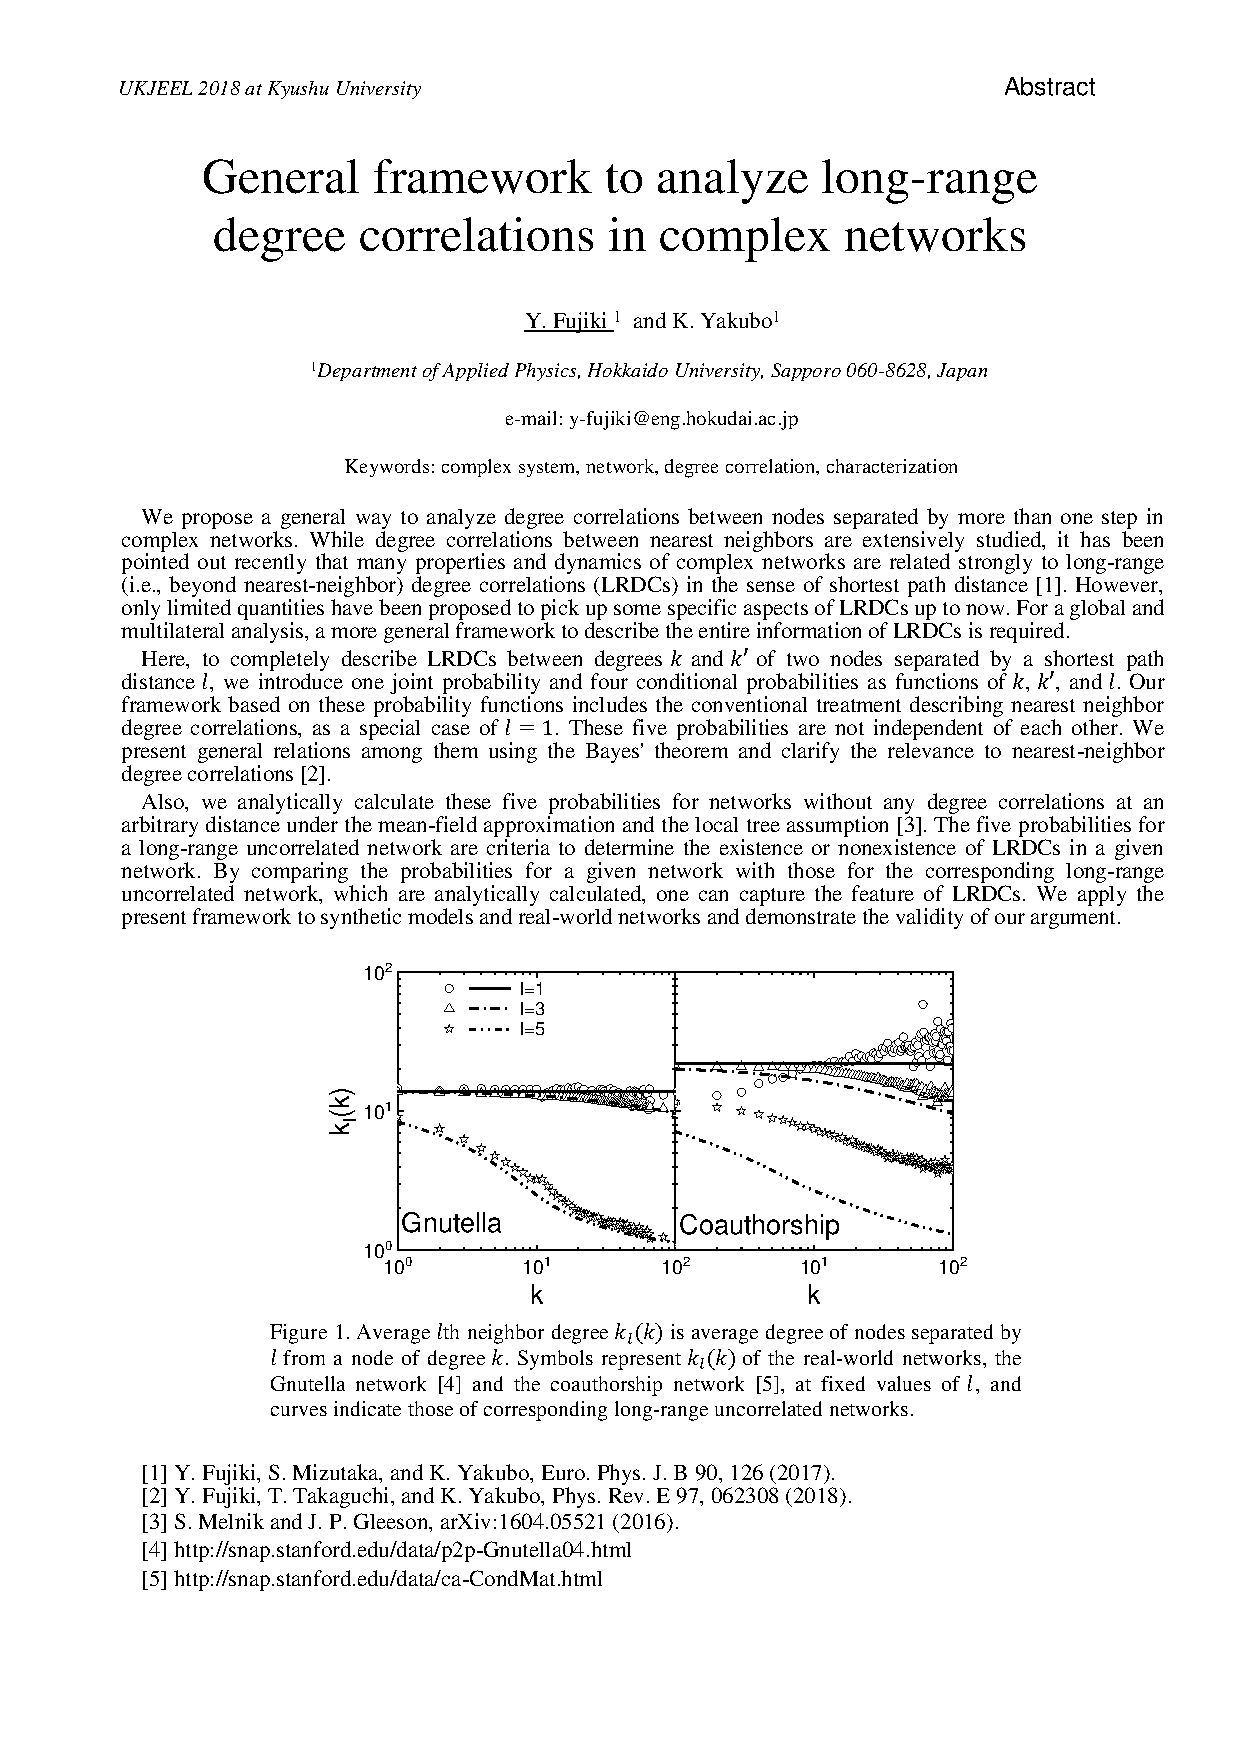
\includepdf[pagecommand={}]{abstracts/24-UKJEEL_Fujiki-Yuka.pdf}

 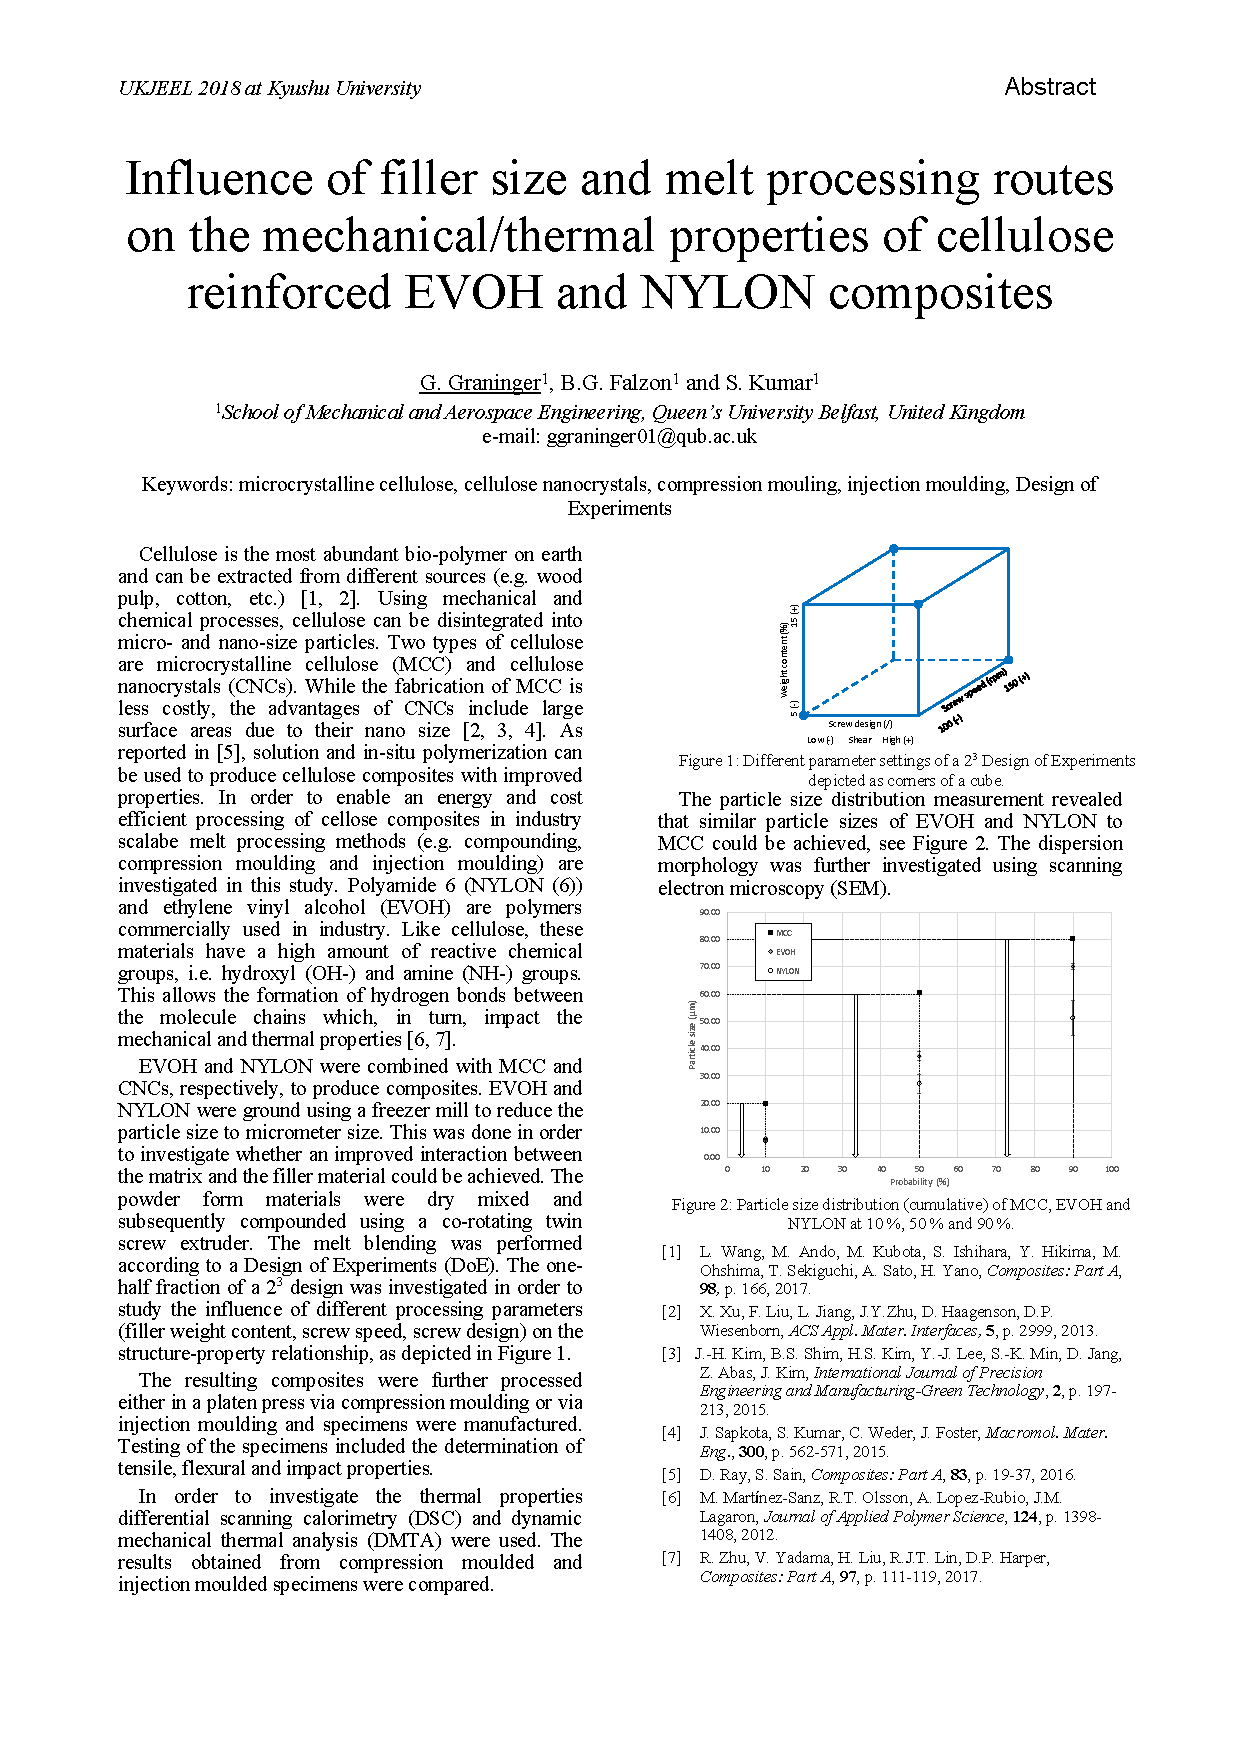
\includepdf[pagecommand={}]{abstracts/04-UKJEEL_Graninger-Georg.pdf}

 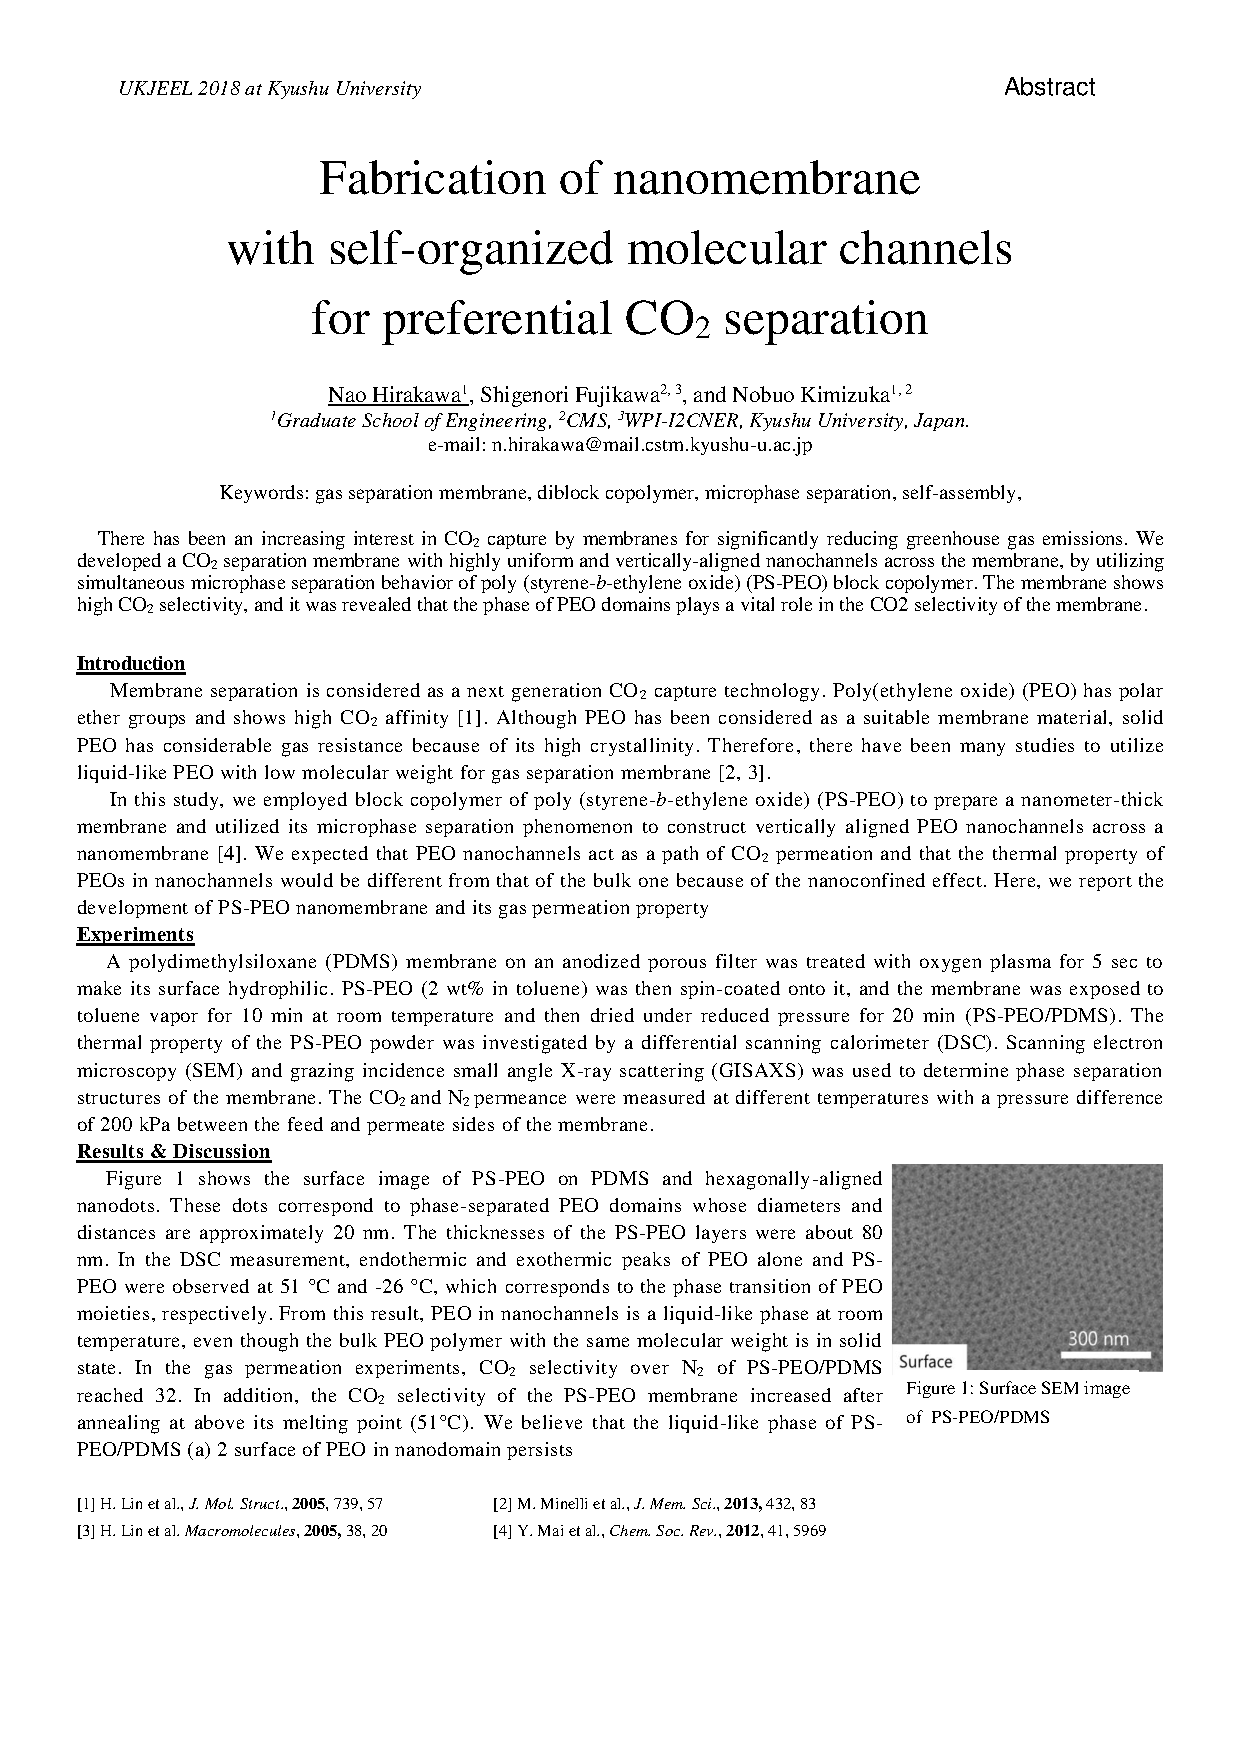
\includepdf[pagecommand={}]{abstracts/14-UKJEEL_Hirakawa-Nao.pdf}

 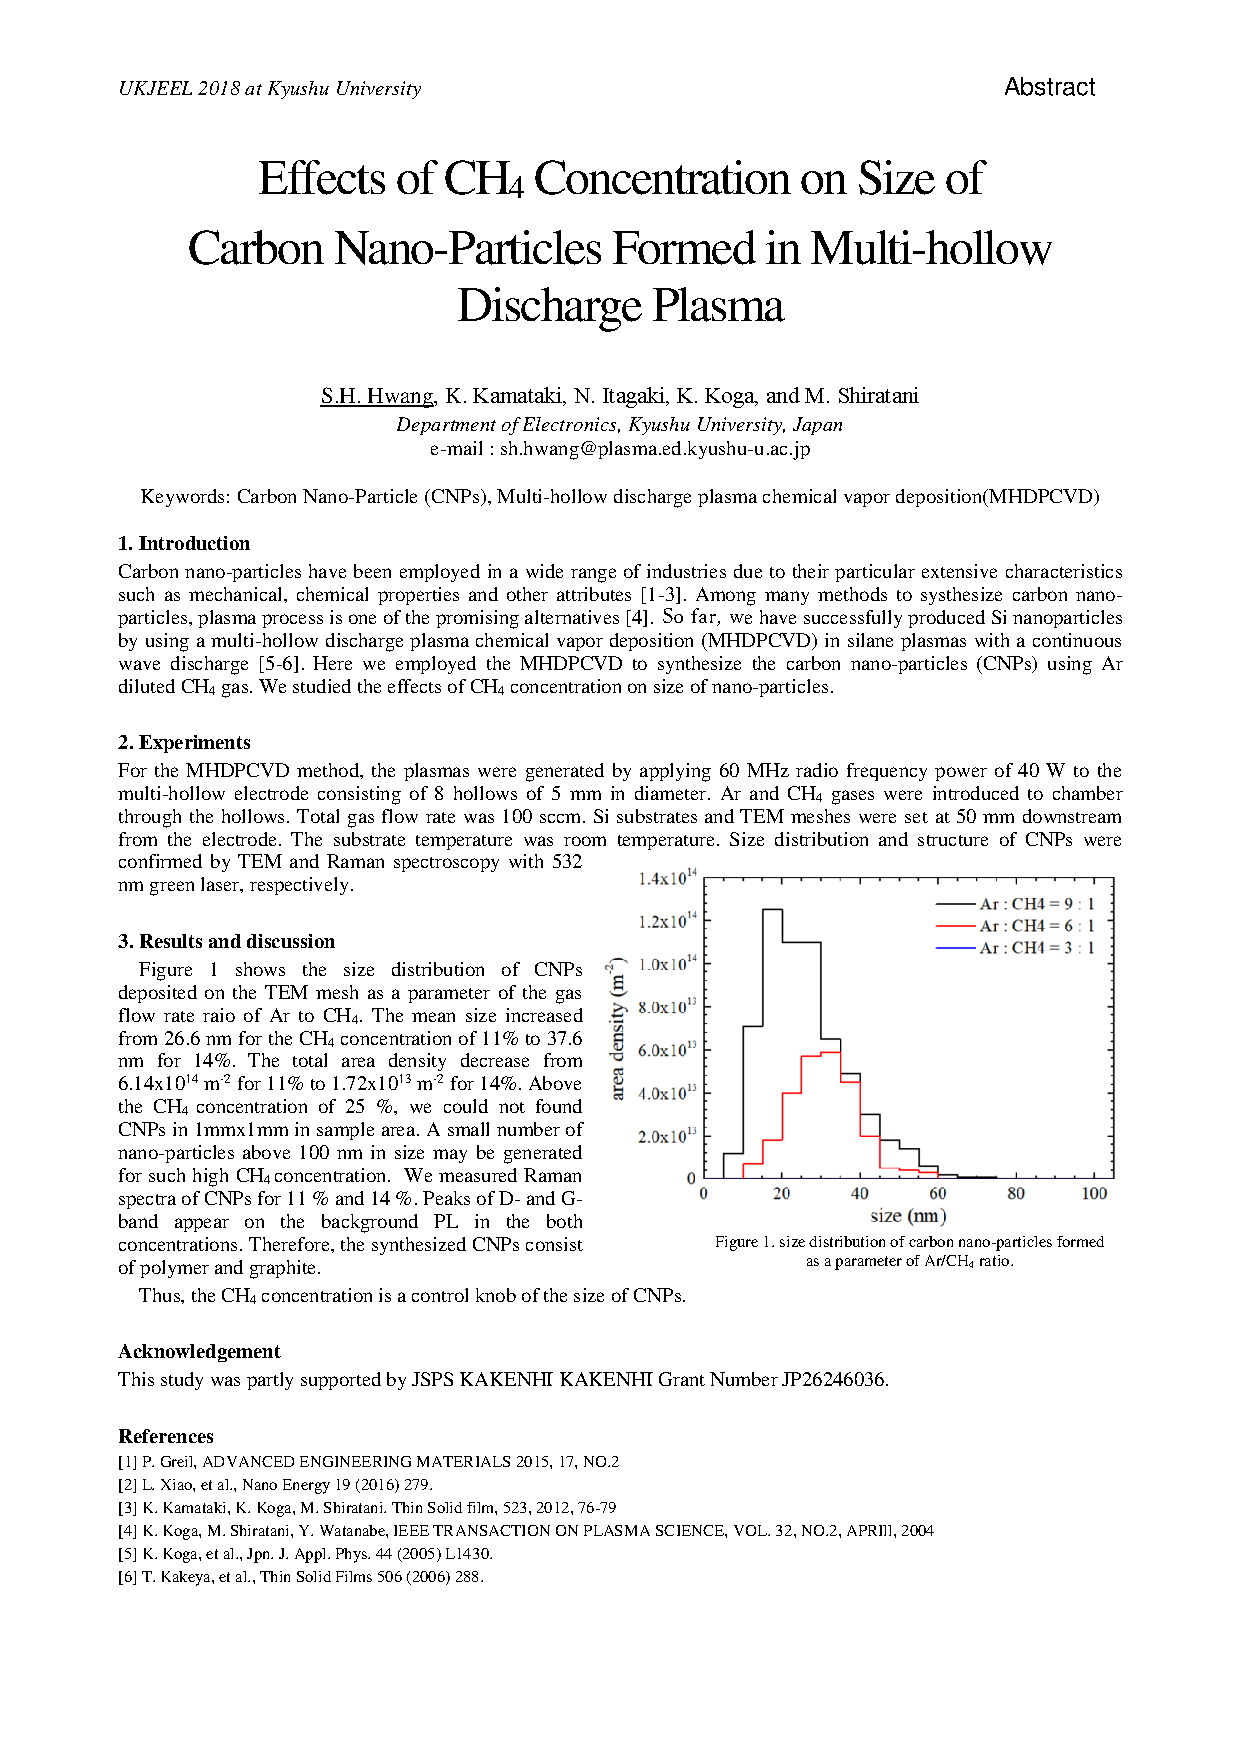
\includepdf[pagecommand={}]{abstracts/11-UKJEEL2018_HWANG_SUNG_HWA.pdf}

 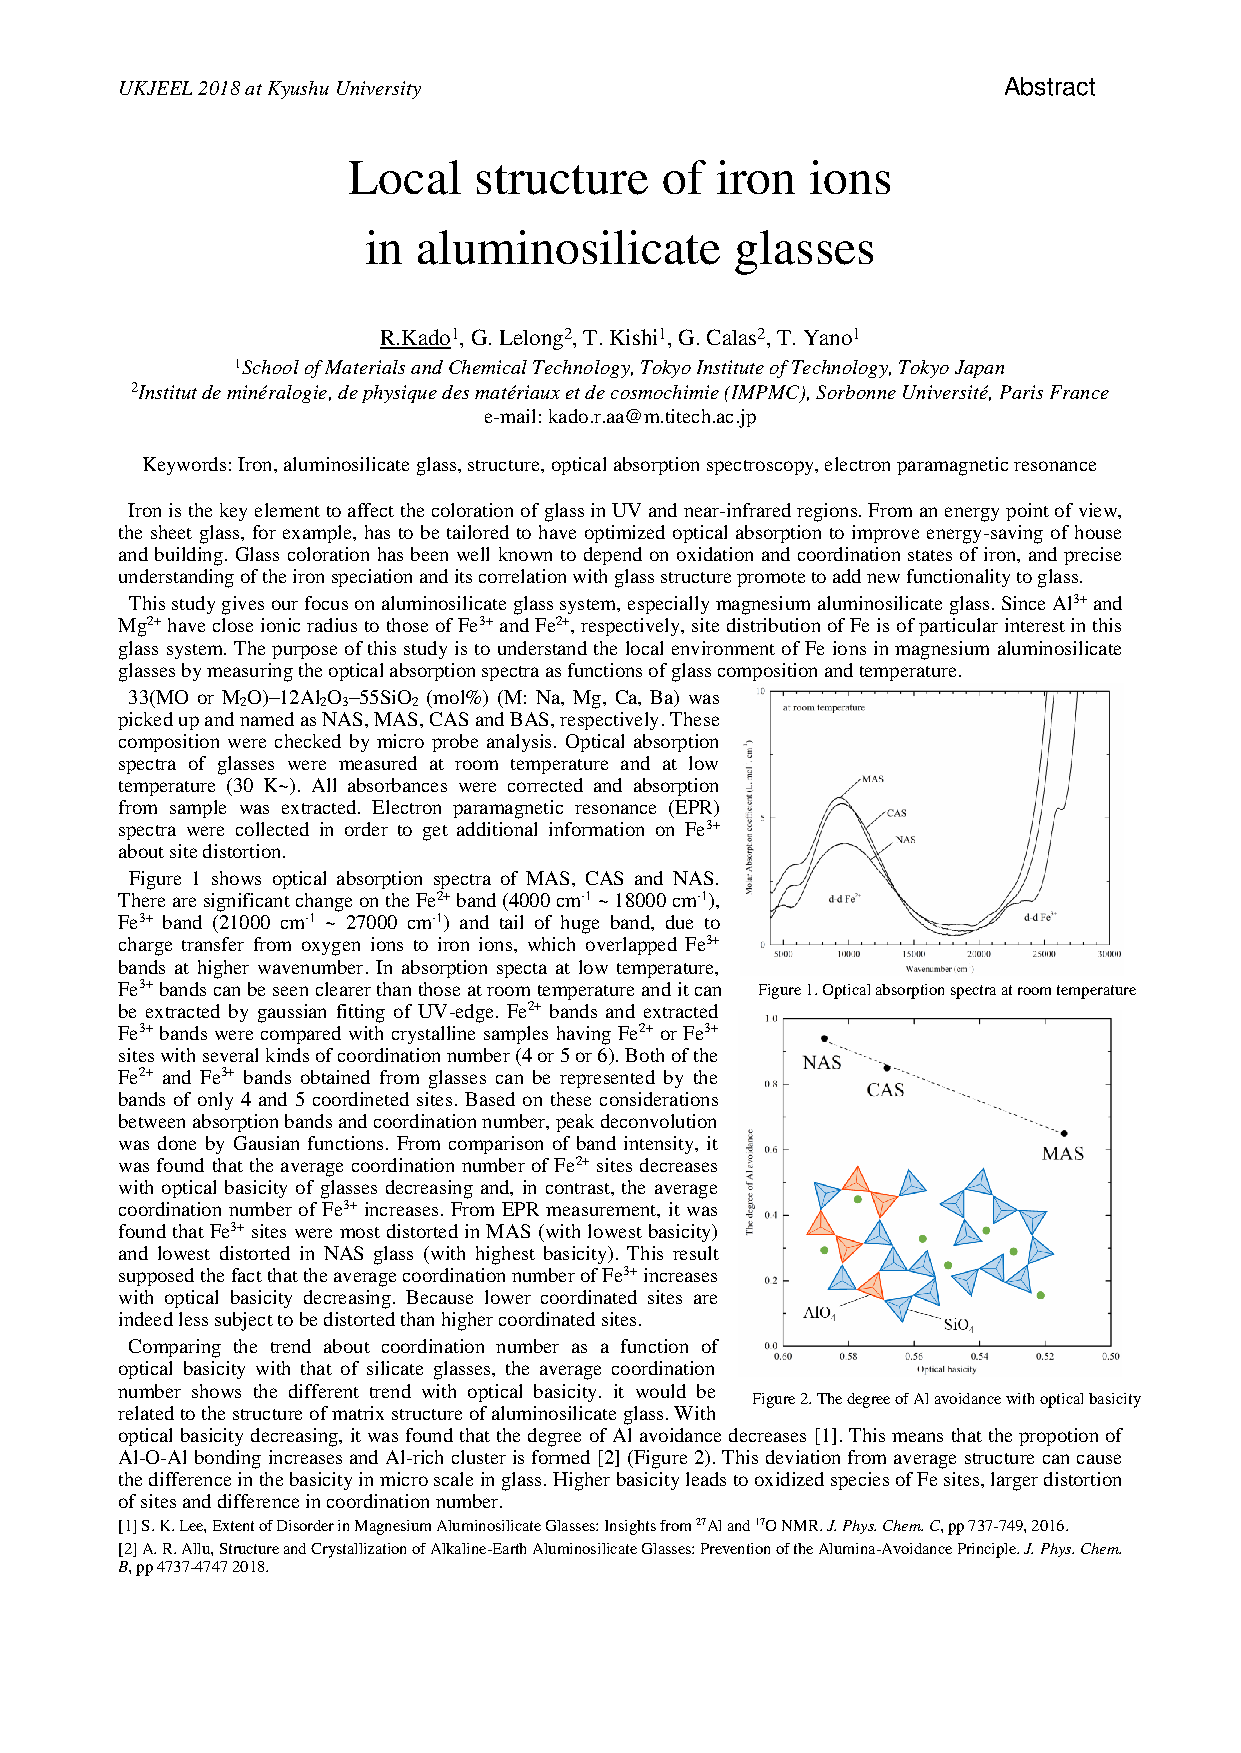
\includepdf[pagecommand={}]{abstracts/25-UKJEEL2018_Rikiya_Kado.pdf}

 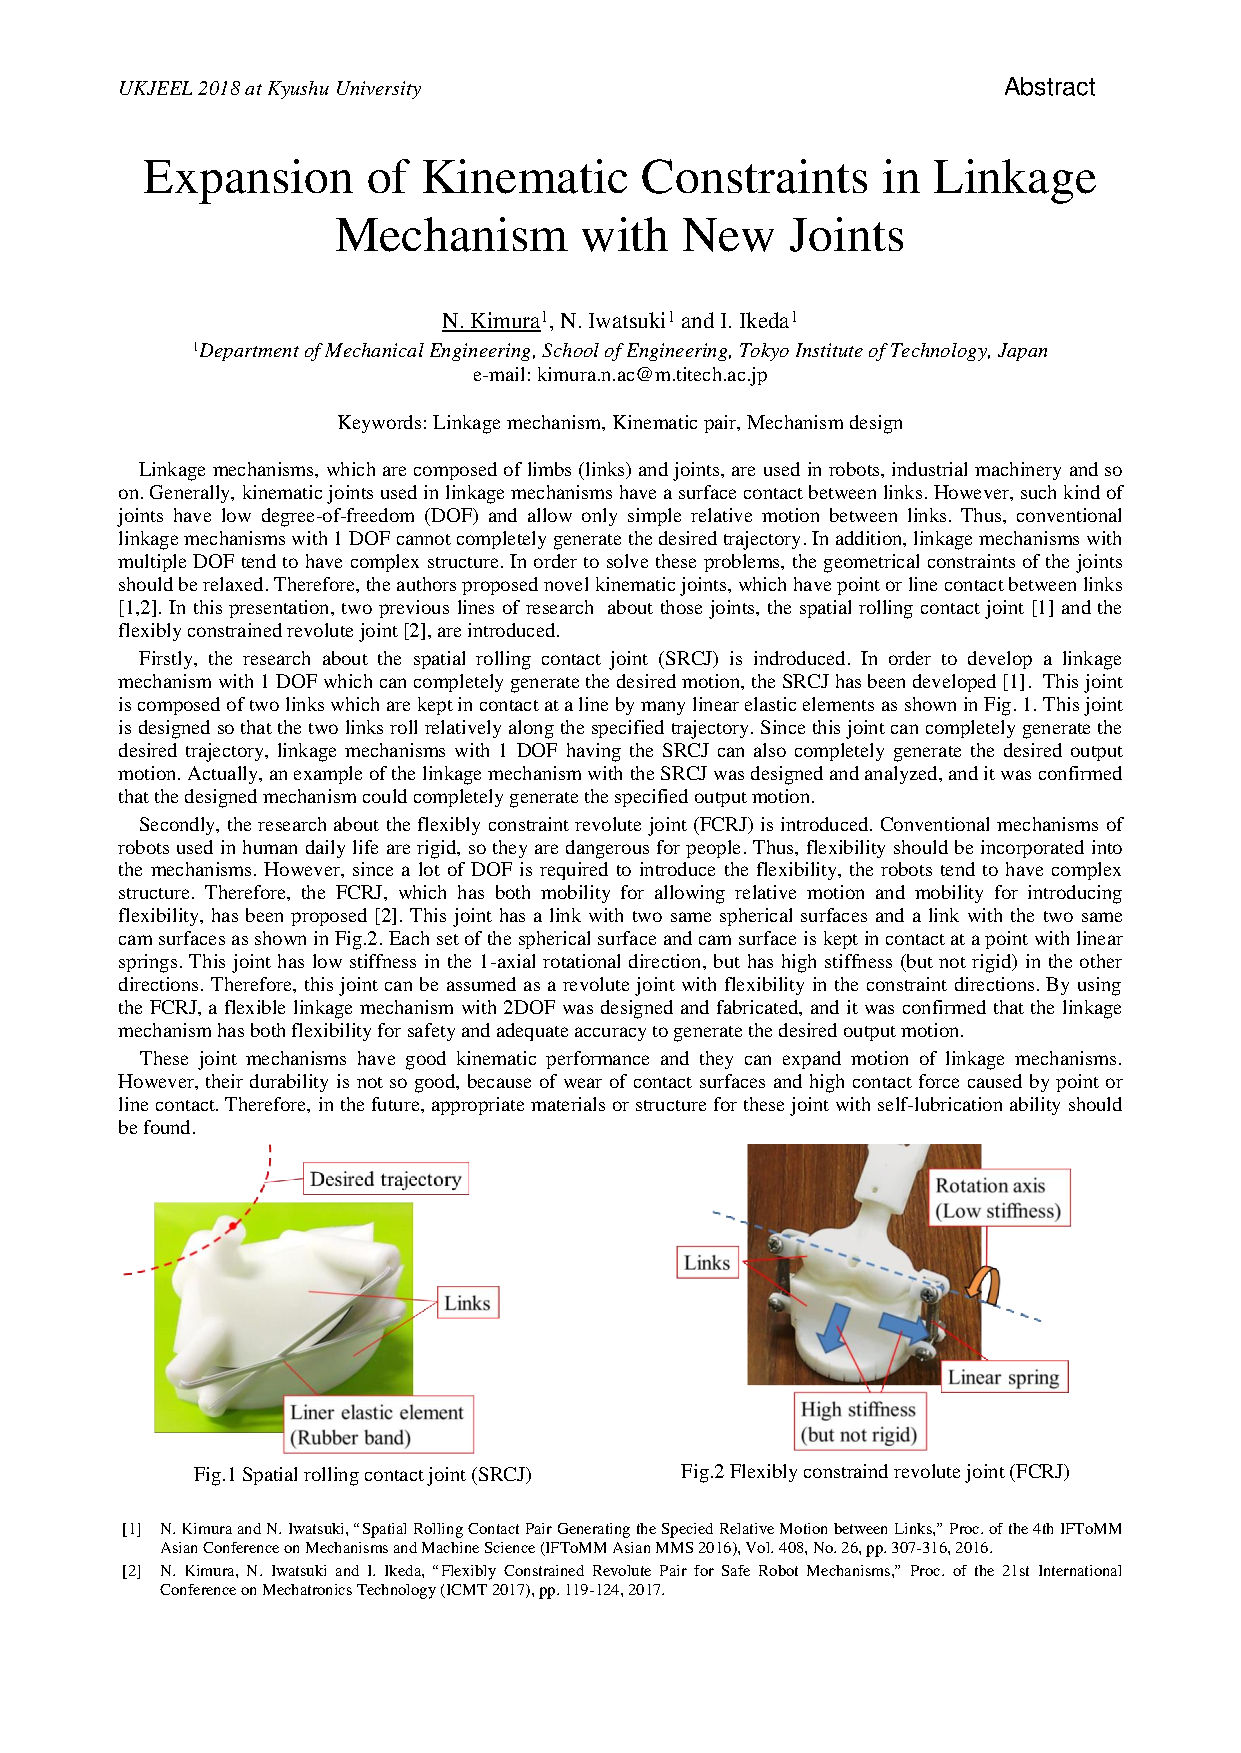
\includepdf[pagecommand={}]{abstracts/13-UKJEEL2018_kimura.pdf}

 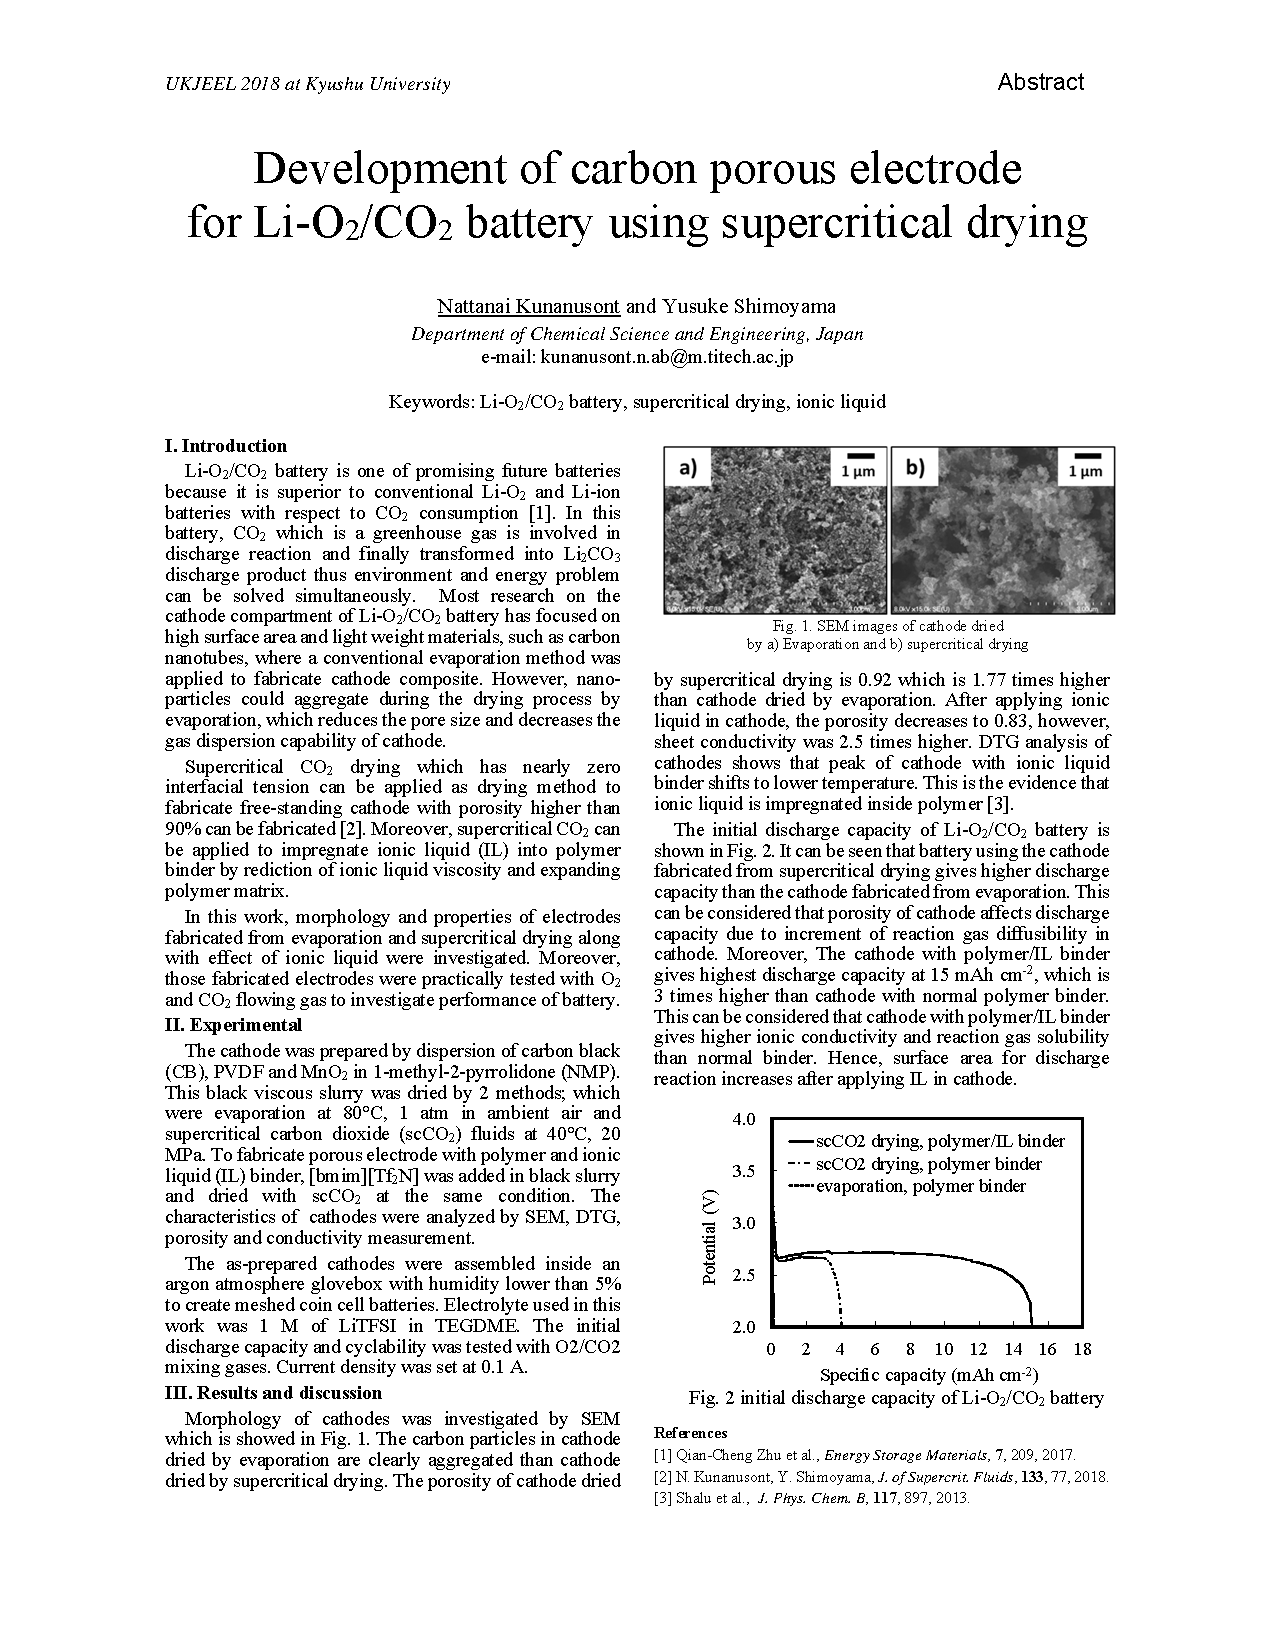
\includepdf[pagecommand={}]{abstracts/22-UKJEEL2018_K_Nattanai.pdf}

 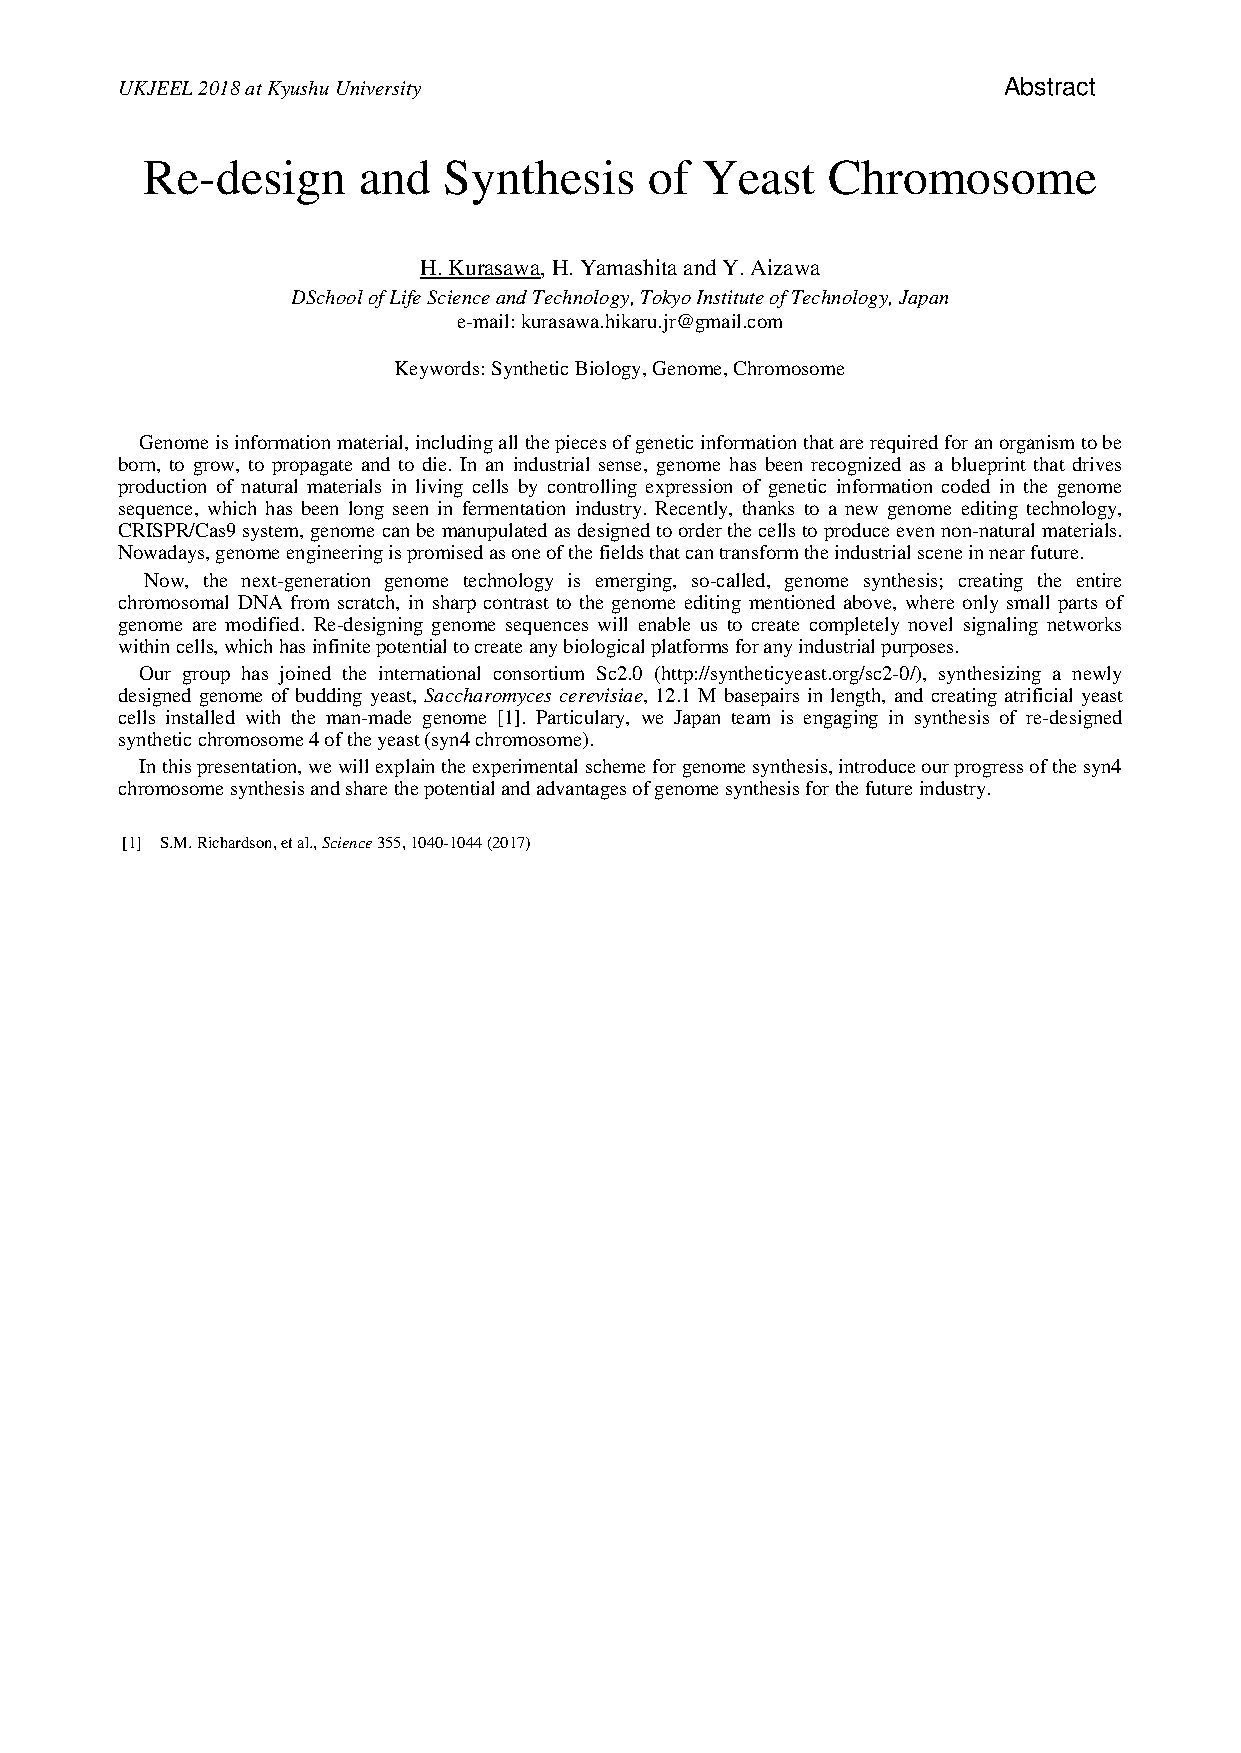
\includepdf[pagecommand={}]{abstracts/27-UKJEEL2018_Kurasawa.pdf}

 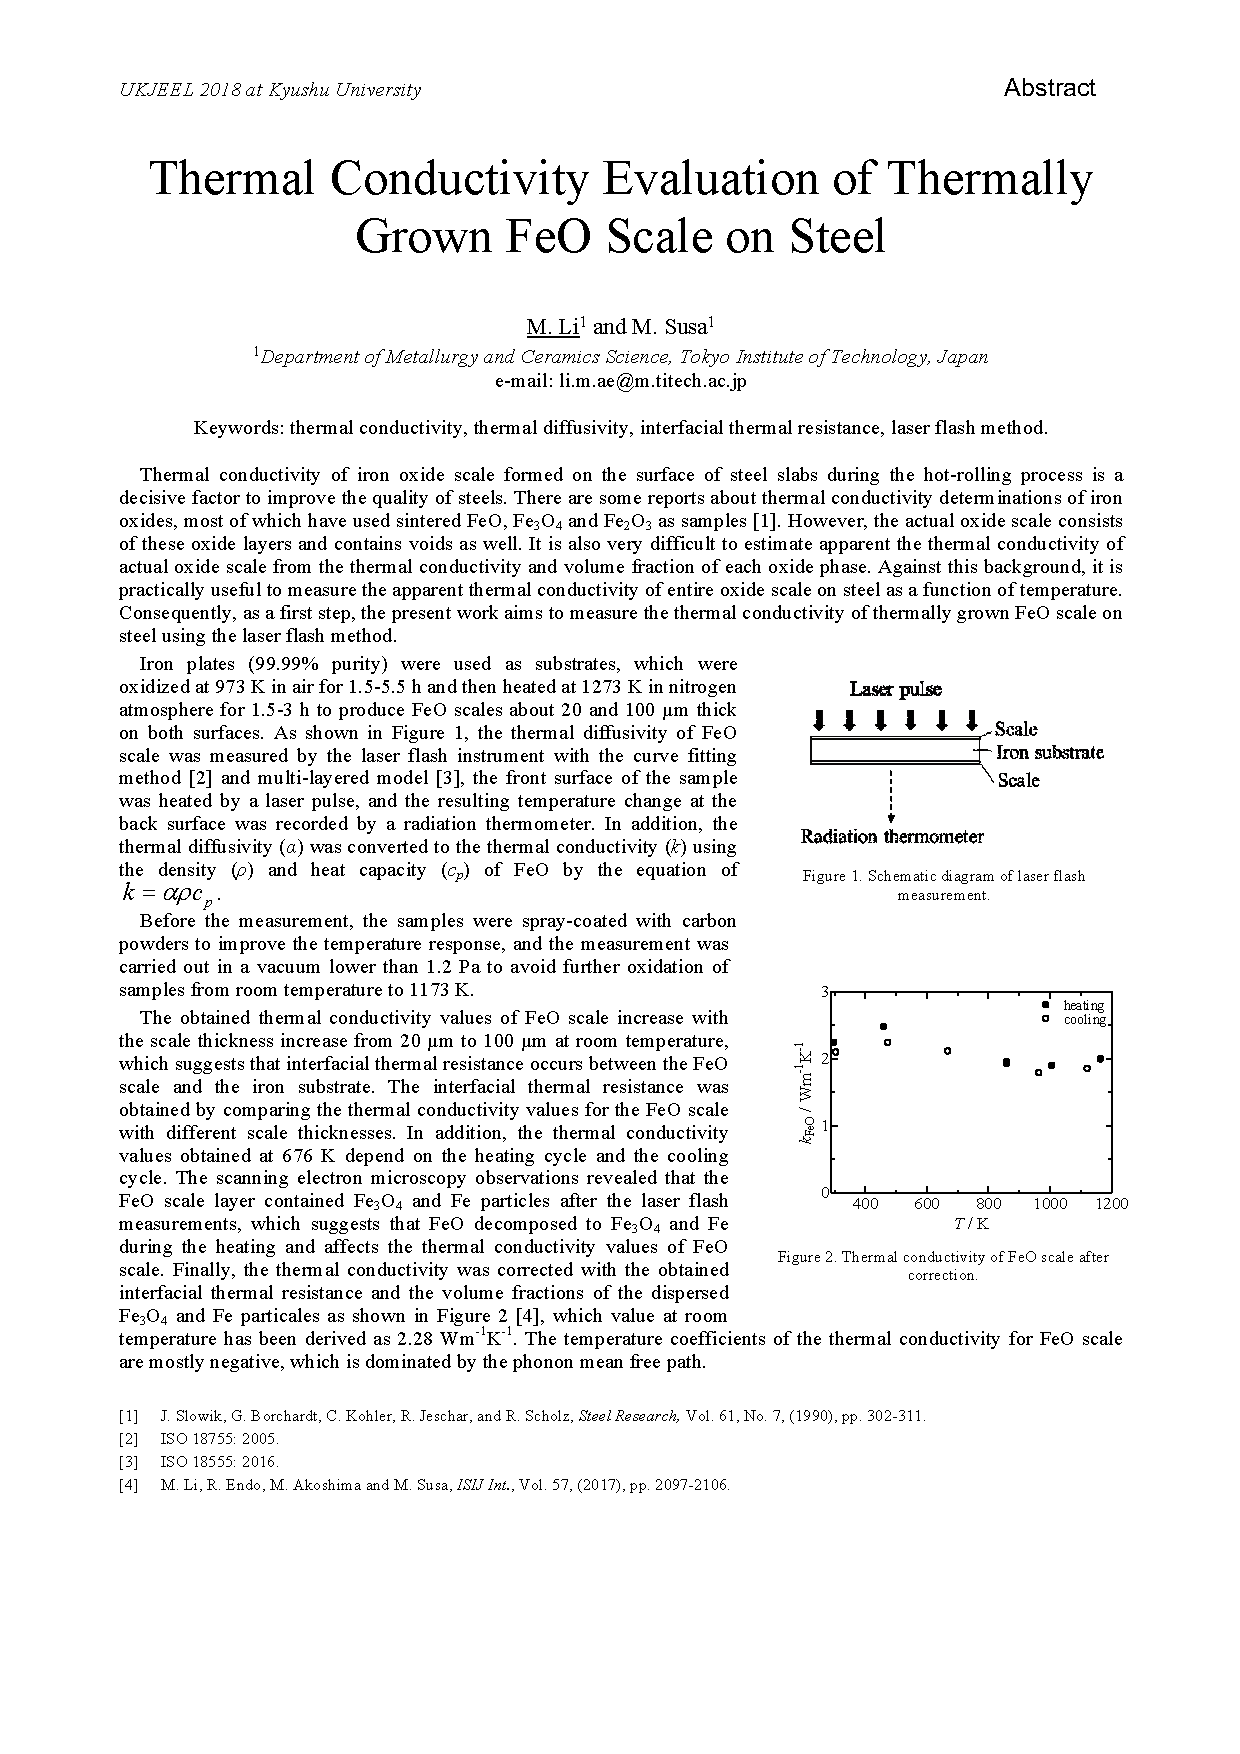
\includepdf[pagecommand={}]{abstracts/21-UKJEEL_Li-Mu.pdf}

 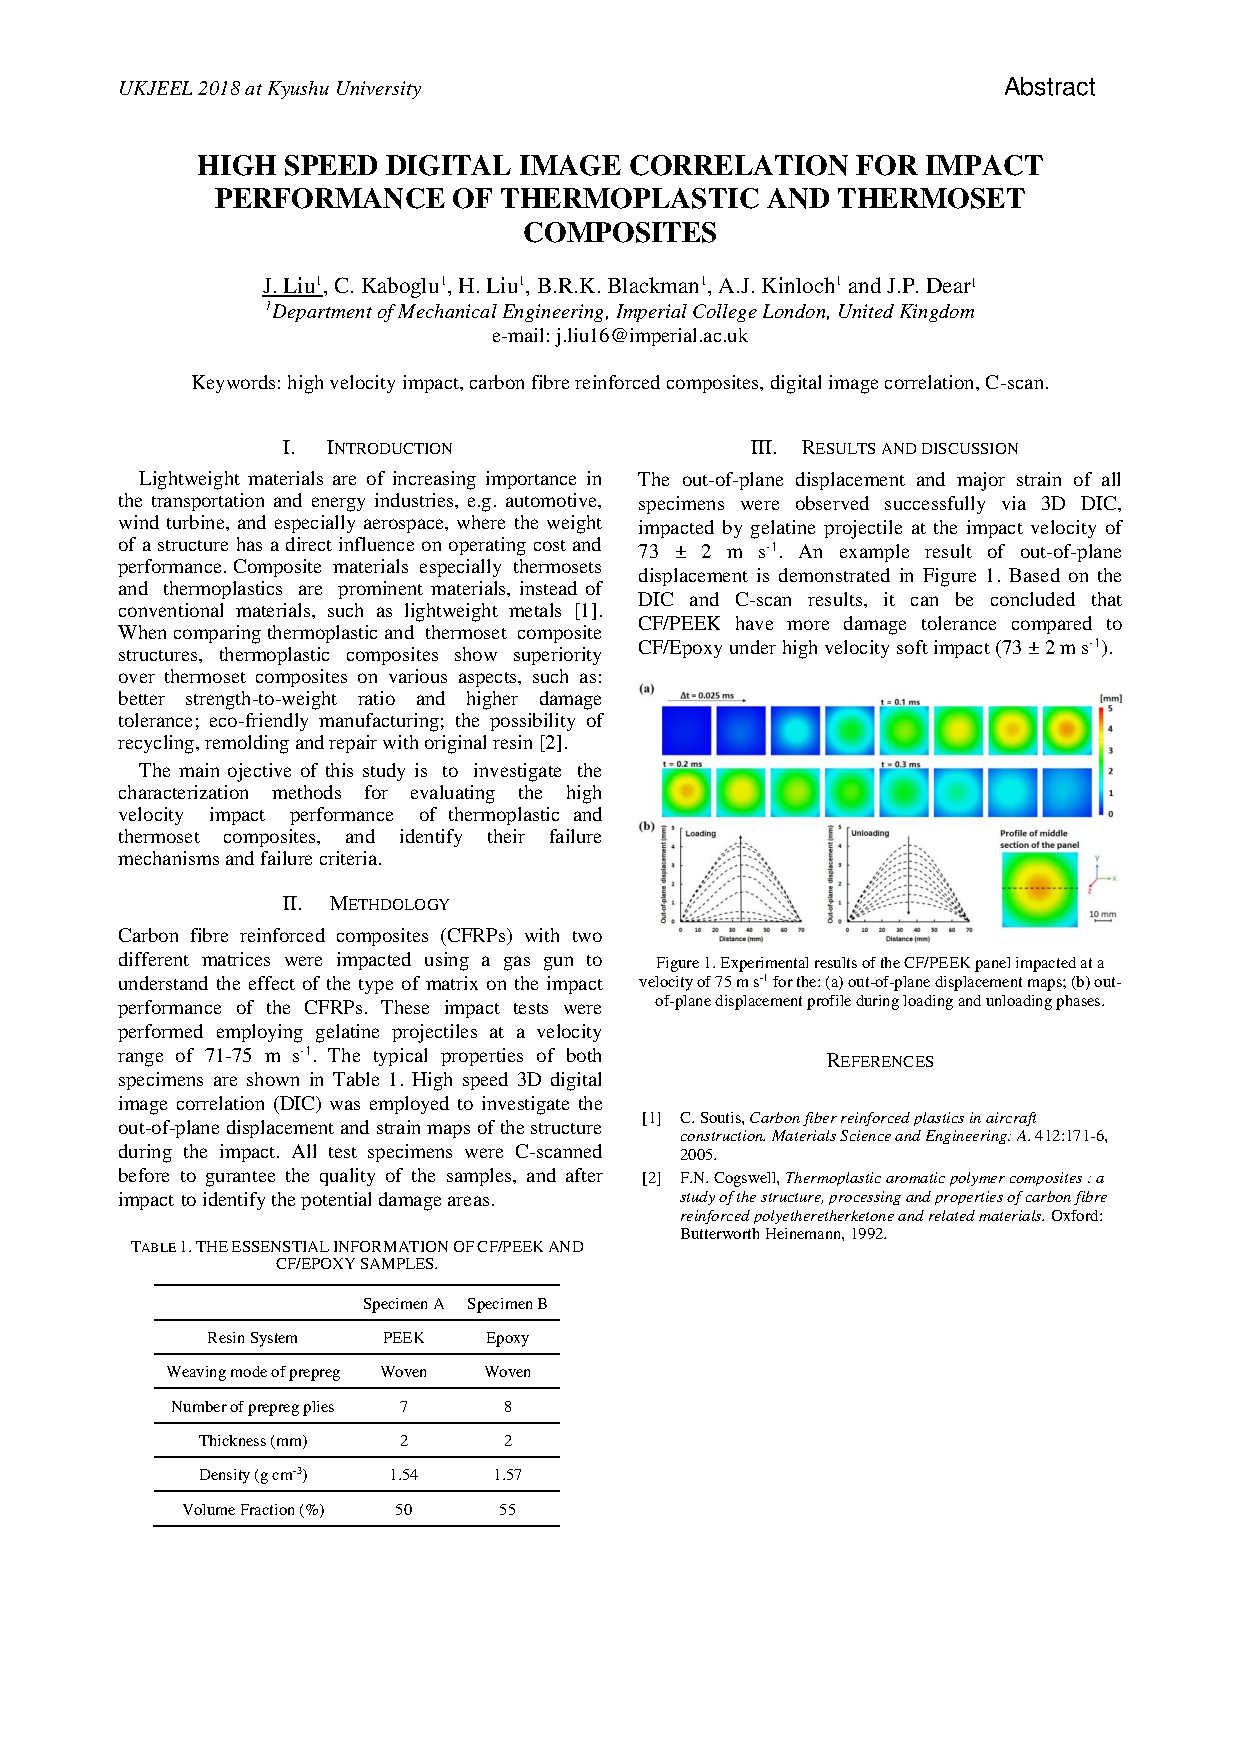
\includepdf[pagecommand={}]{abstracts/20-UKJEEL_Liu-Jun.pdf}

 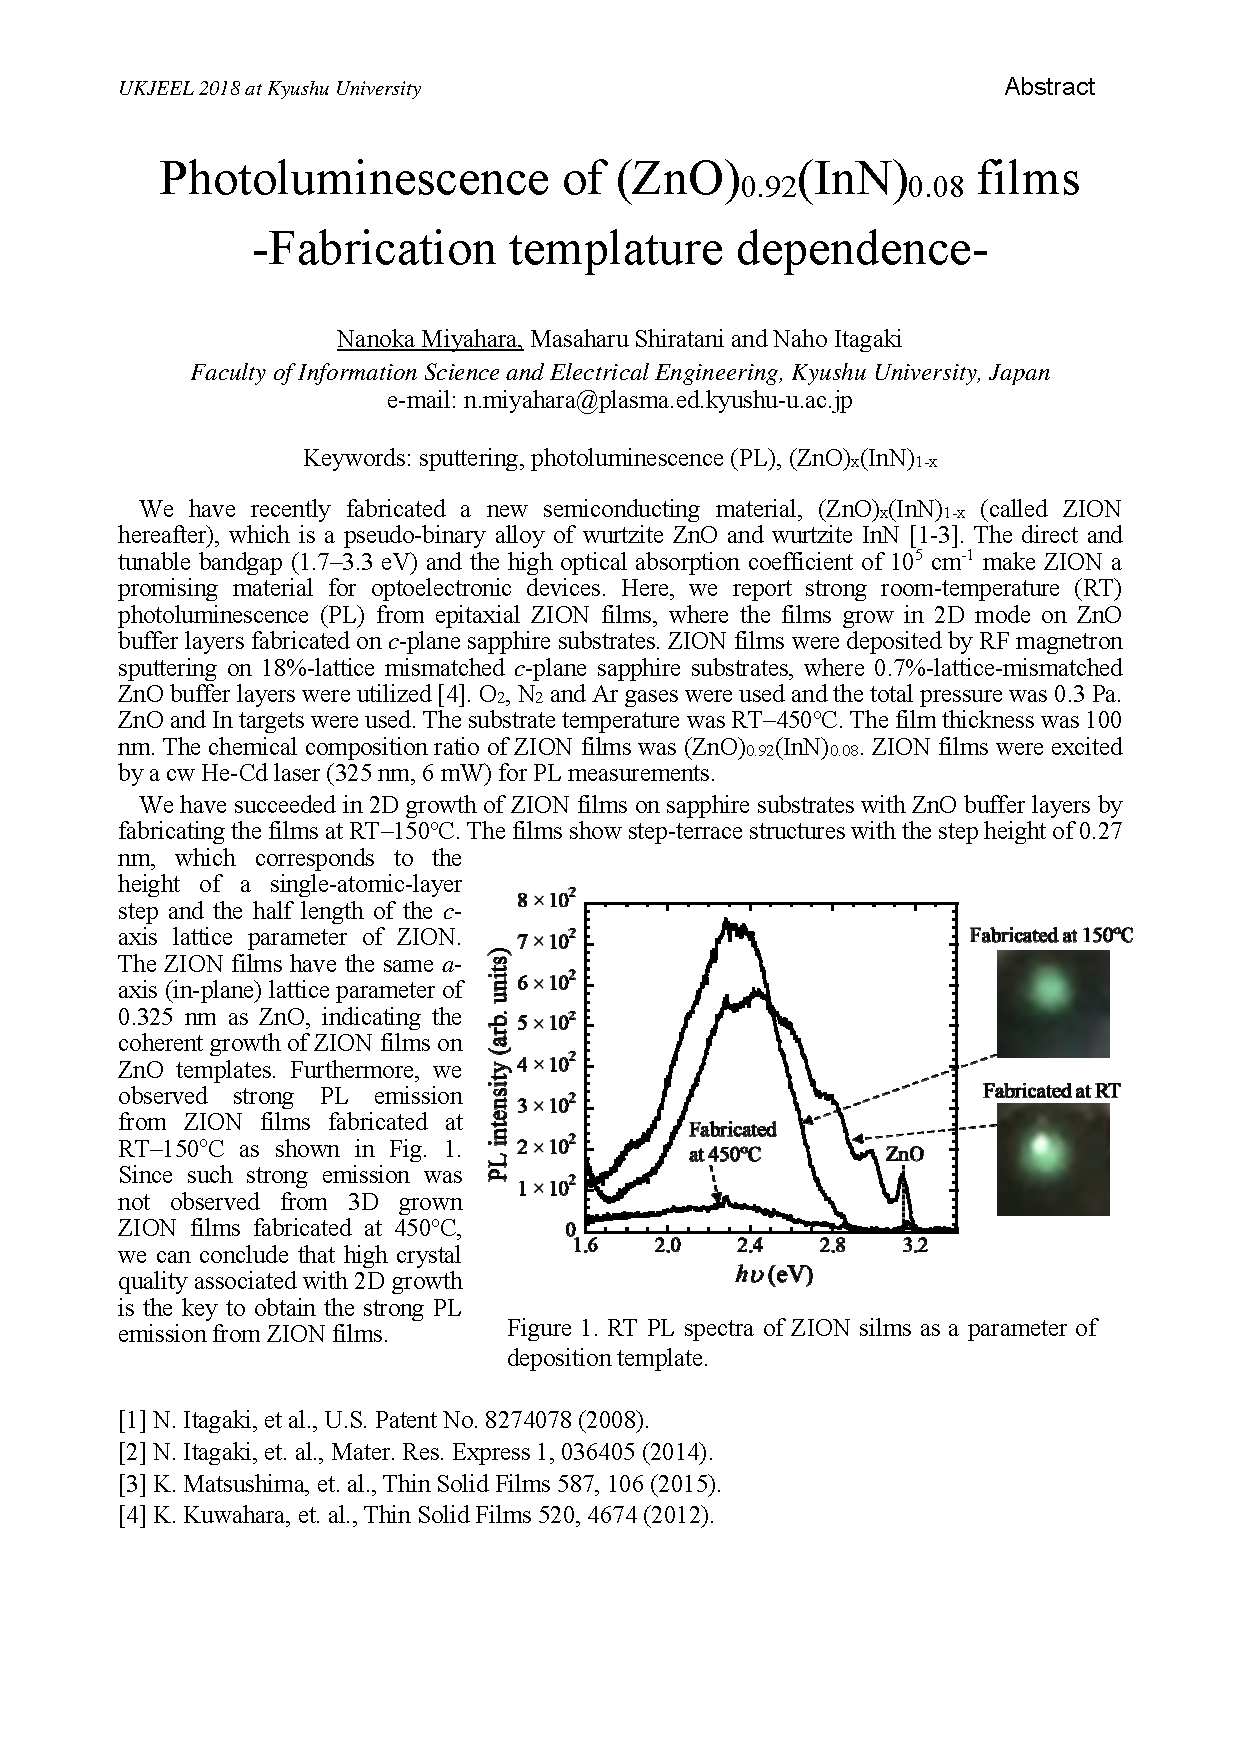
\includepdf[pagecommand={}]{abstracts/09-UKJEEL2018_miyahara_final.pdf}

 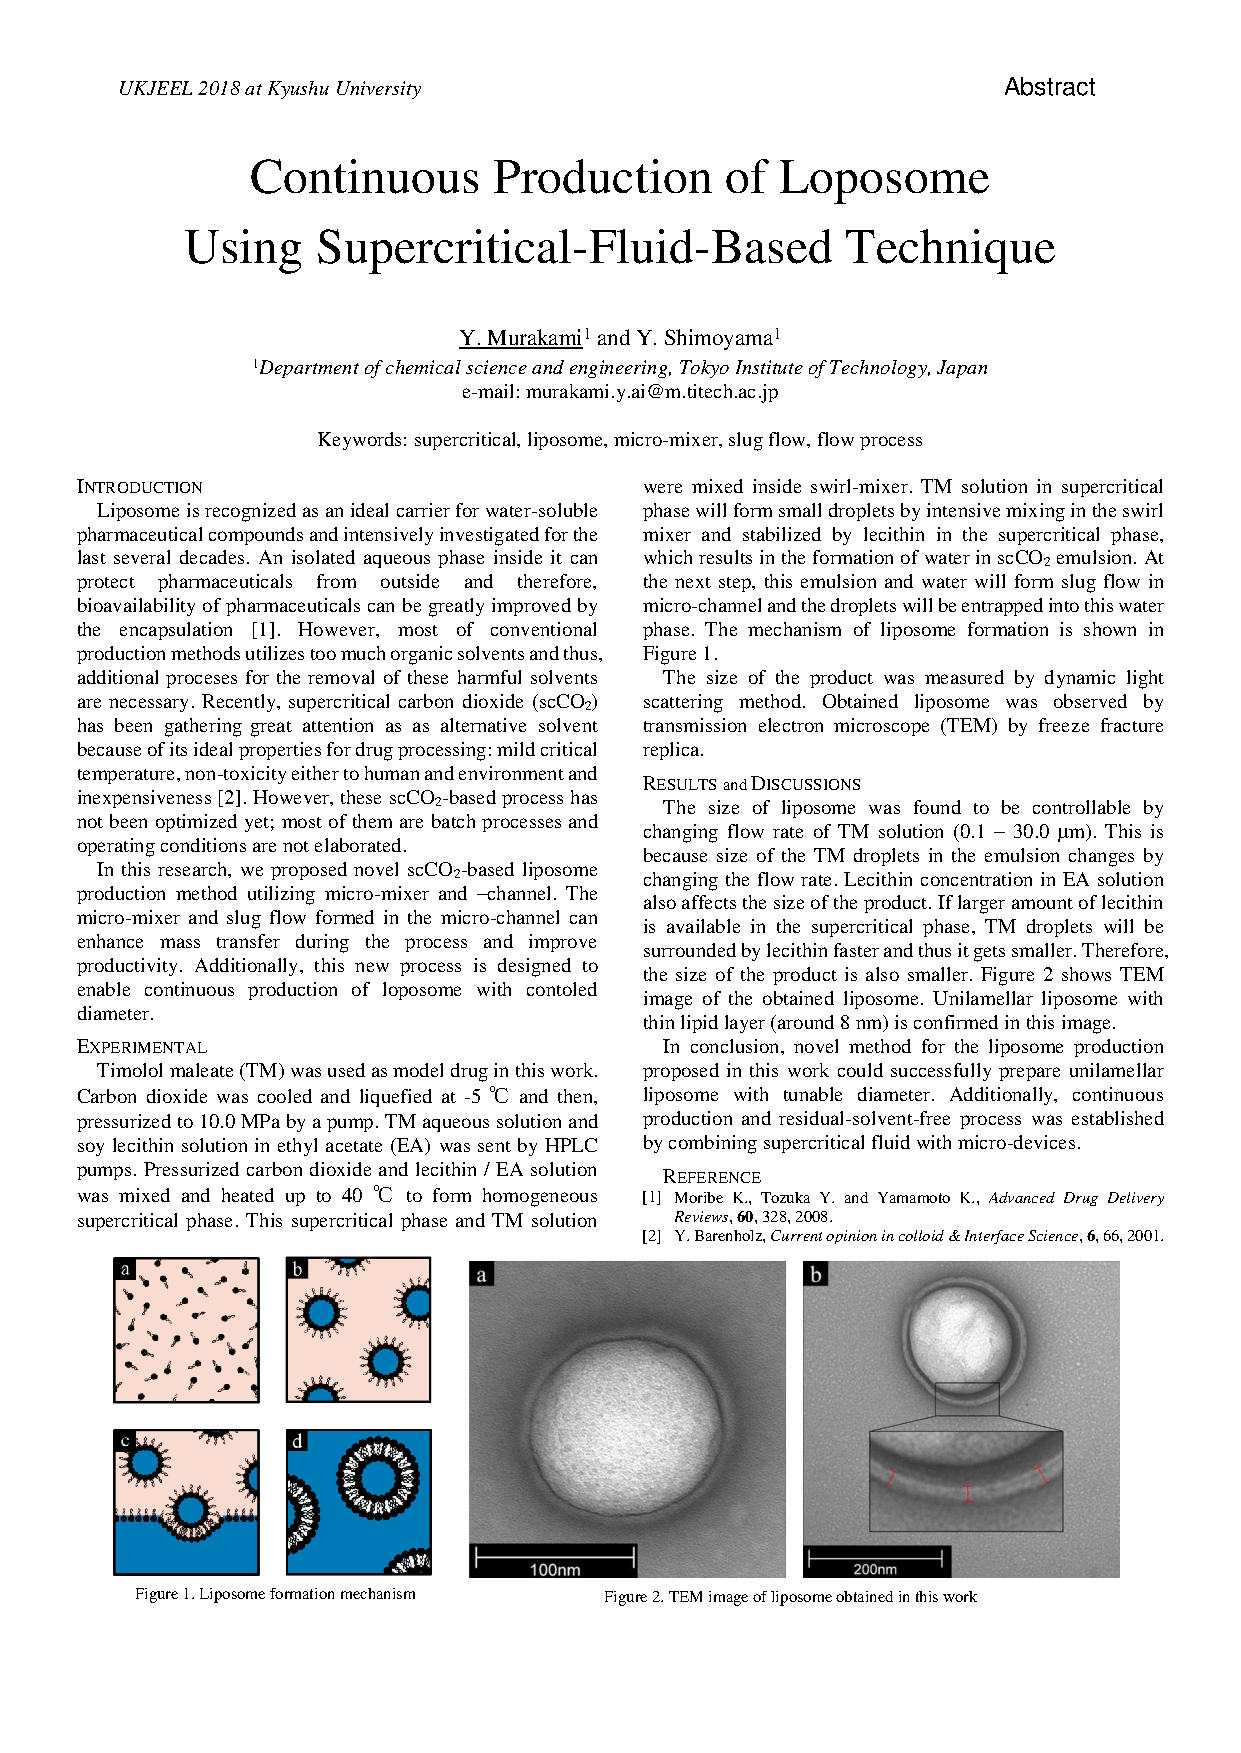
\includepdf[pagecommand={}]{abstracts/23-UKJEEL2018_Murakami.pdf}

 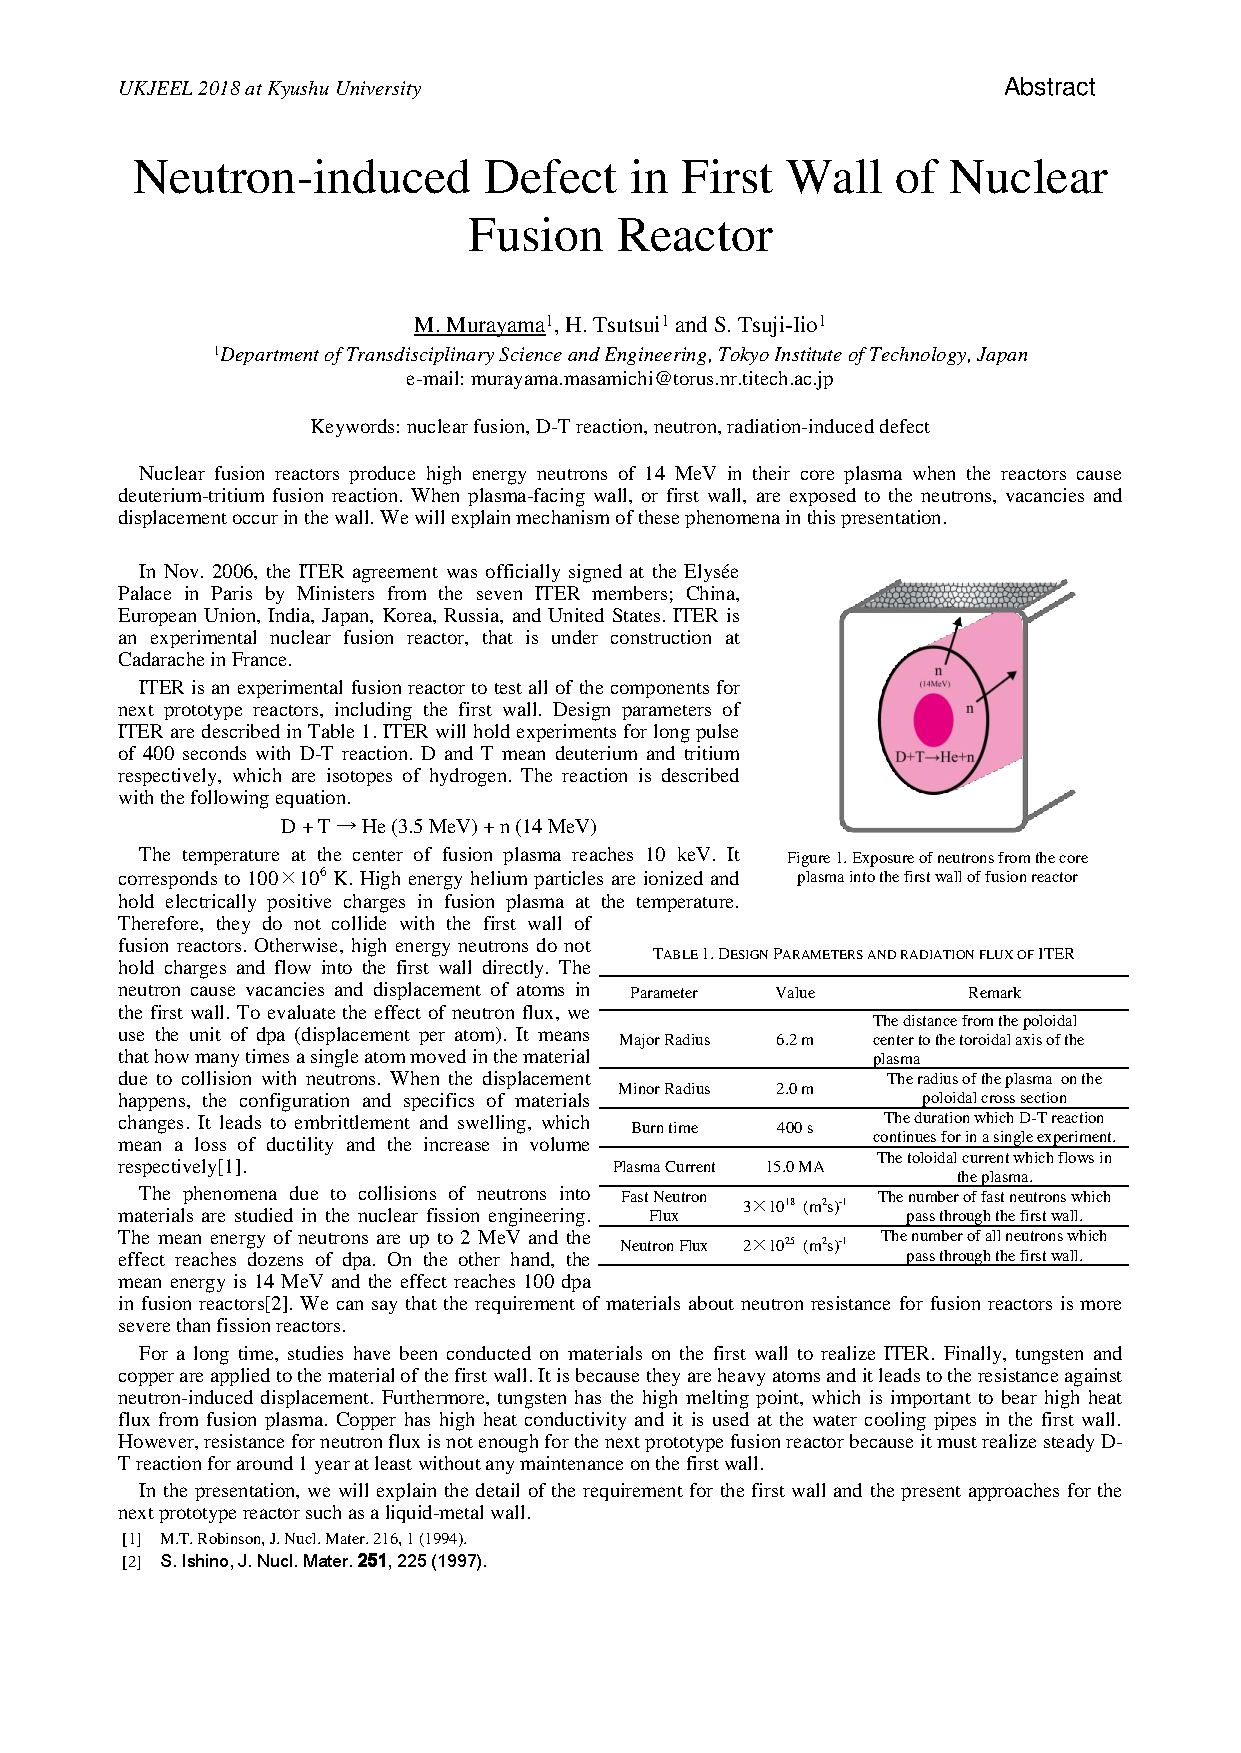
\includepdf[pagecommand={}]{abstracts/26-UKJEEL2018_MasamichiMurayama.pdf}

 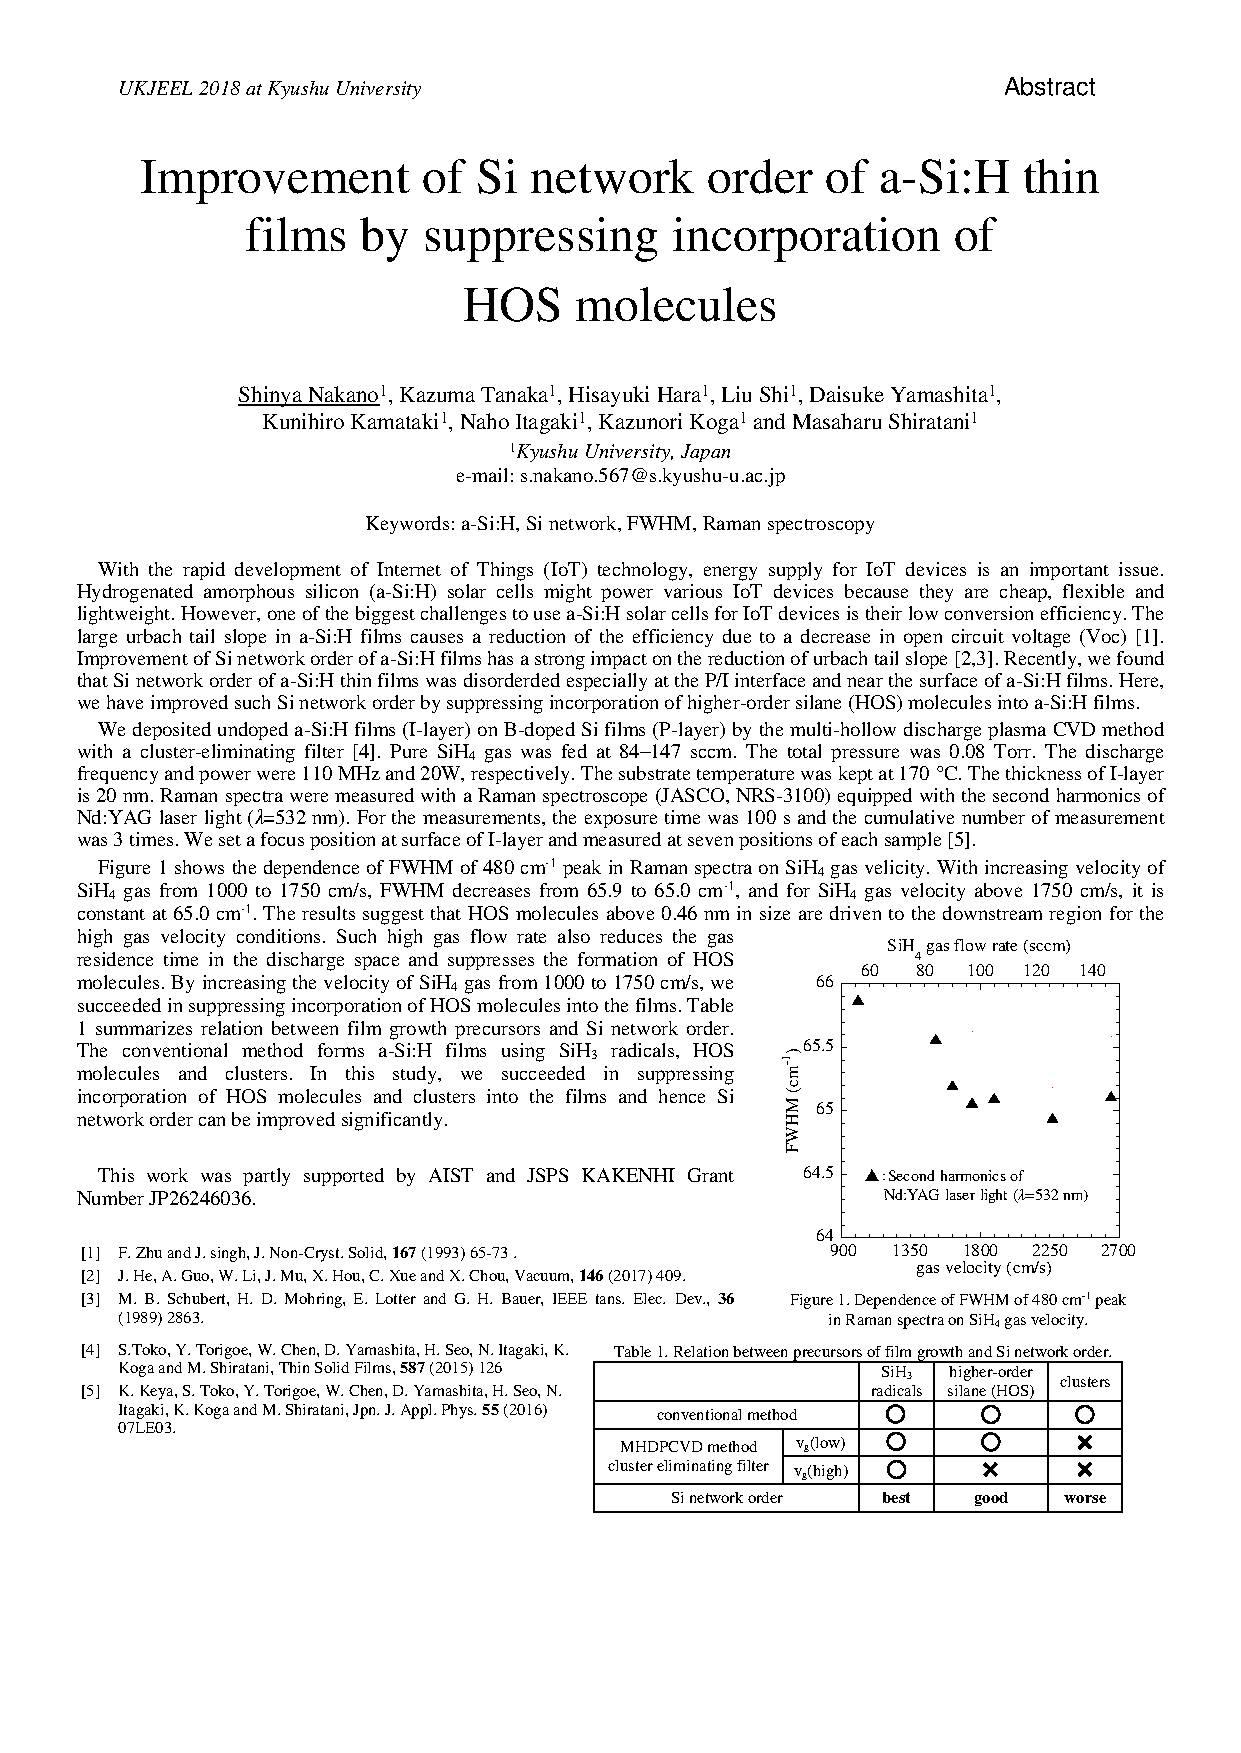
\includepdf[pagecommand={}]{abstracts/10-UKJEEL2018_Nakano.pdf}

 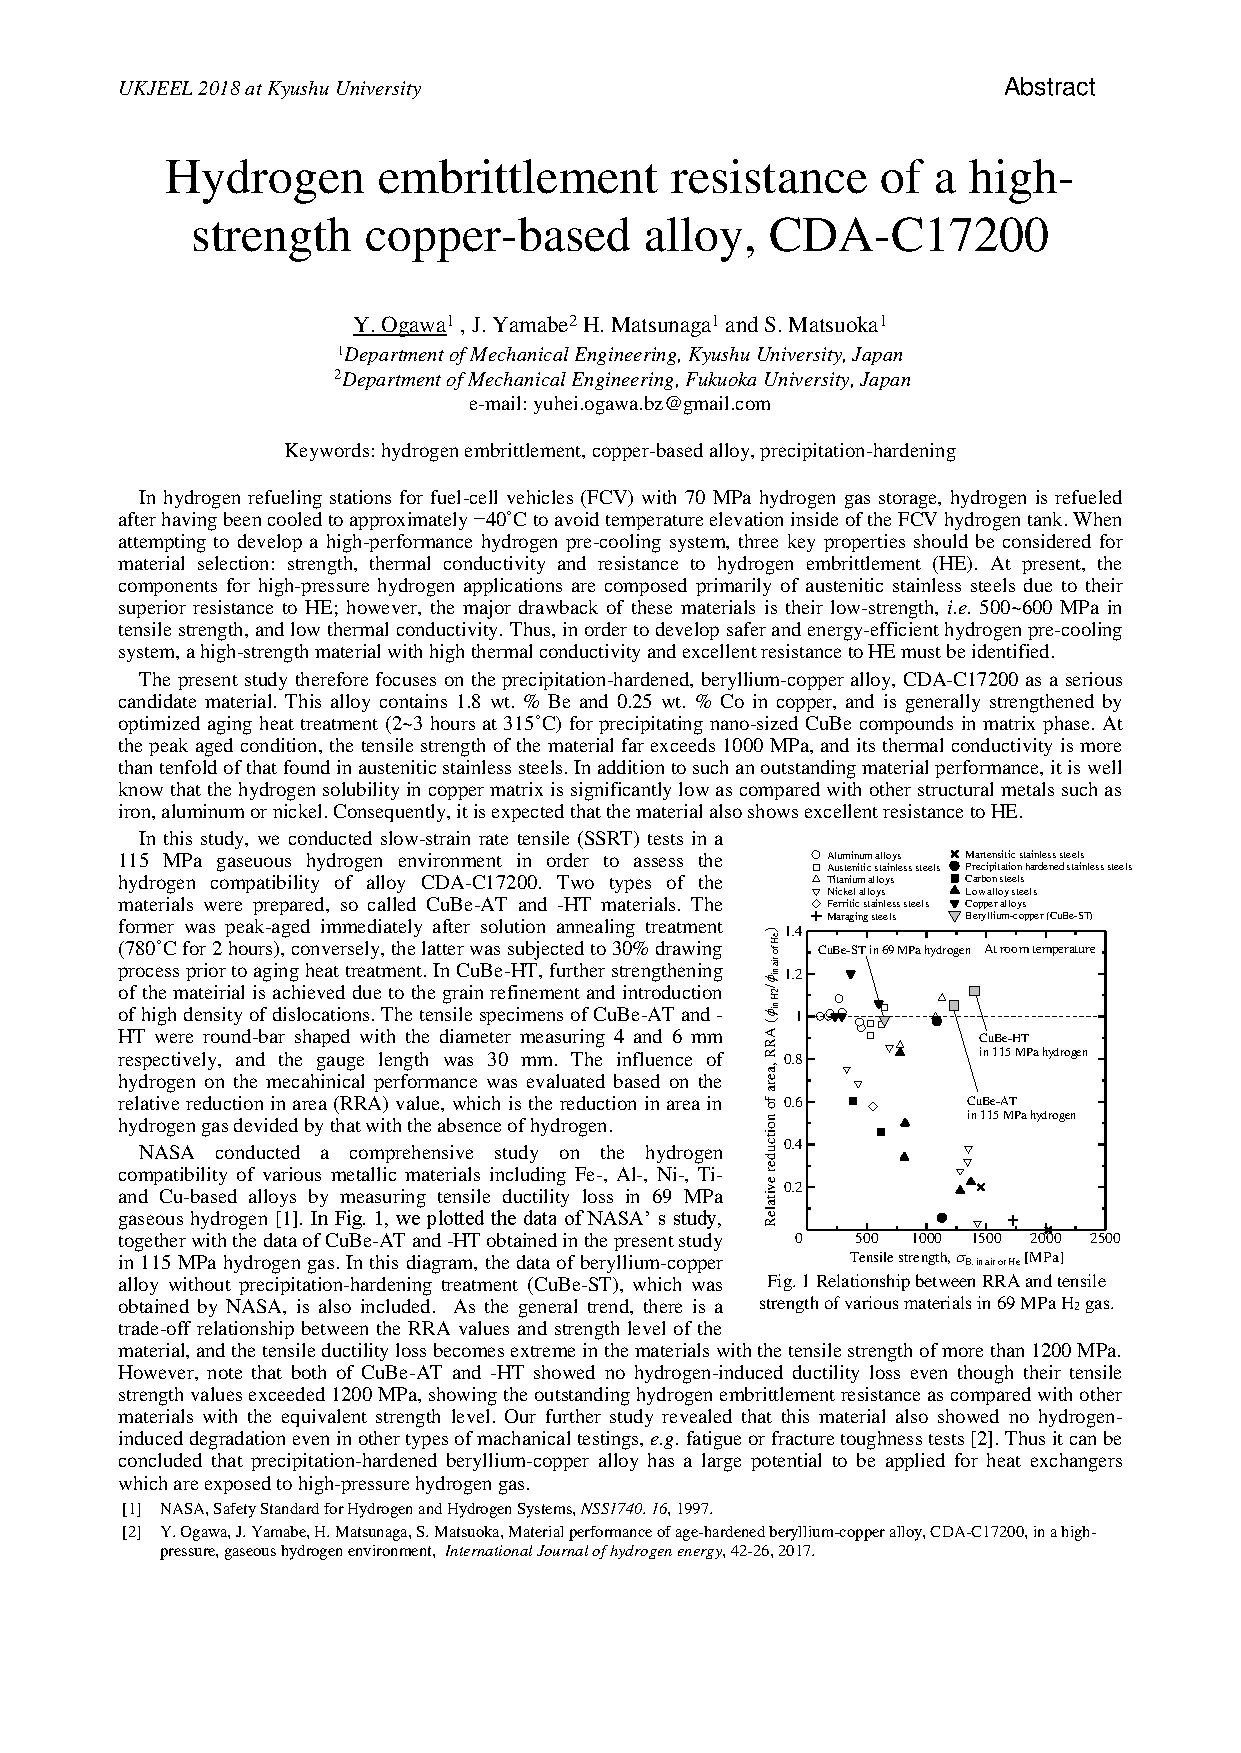
\includepdf[pagecommand={}]{abstracts/15-UKJEEL2018_Ogawa-Yuhei.pdf}

 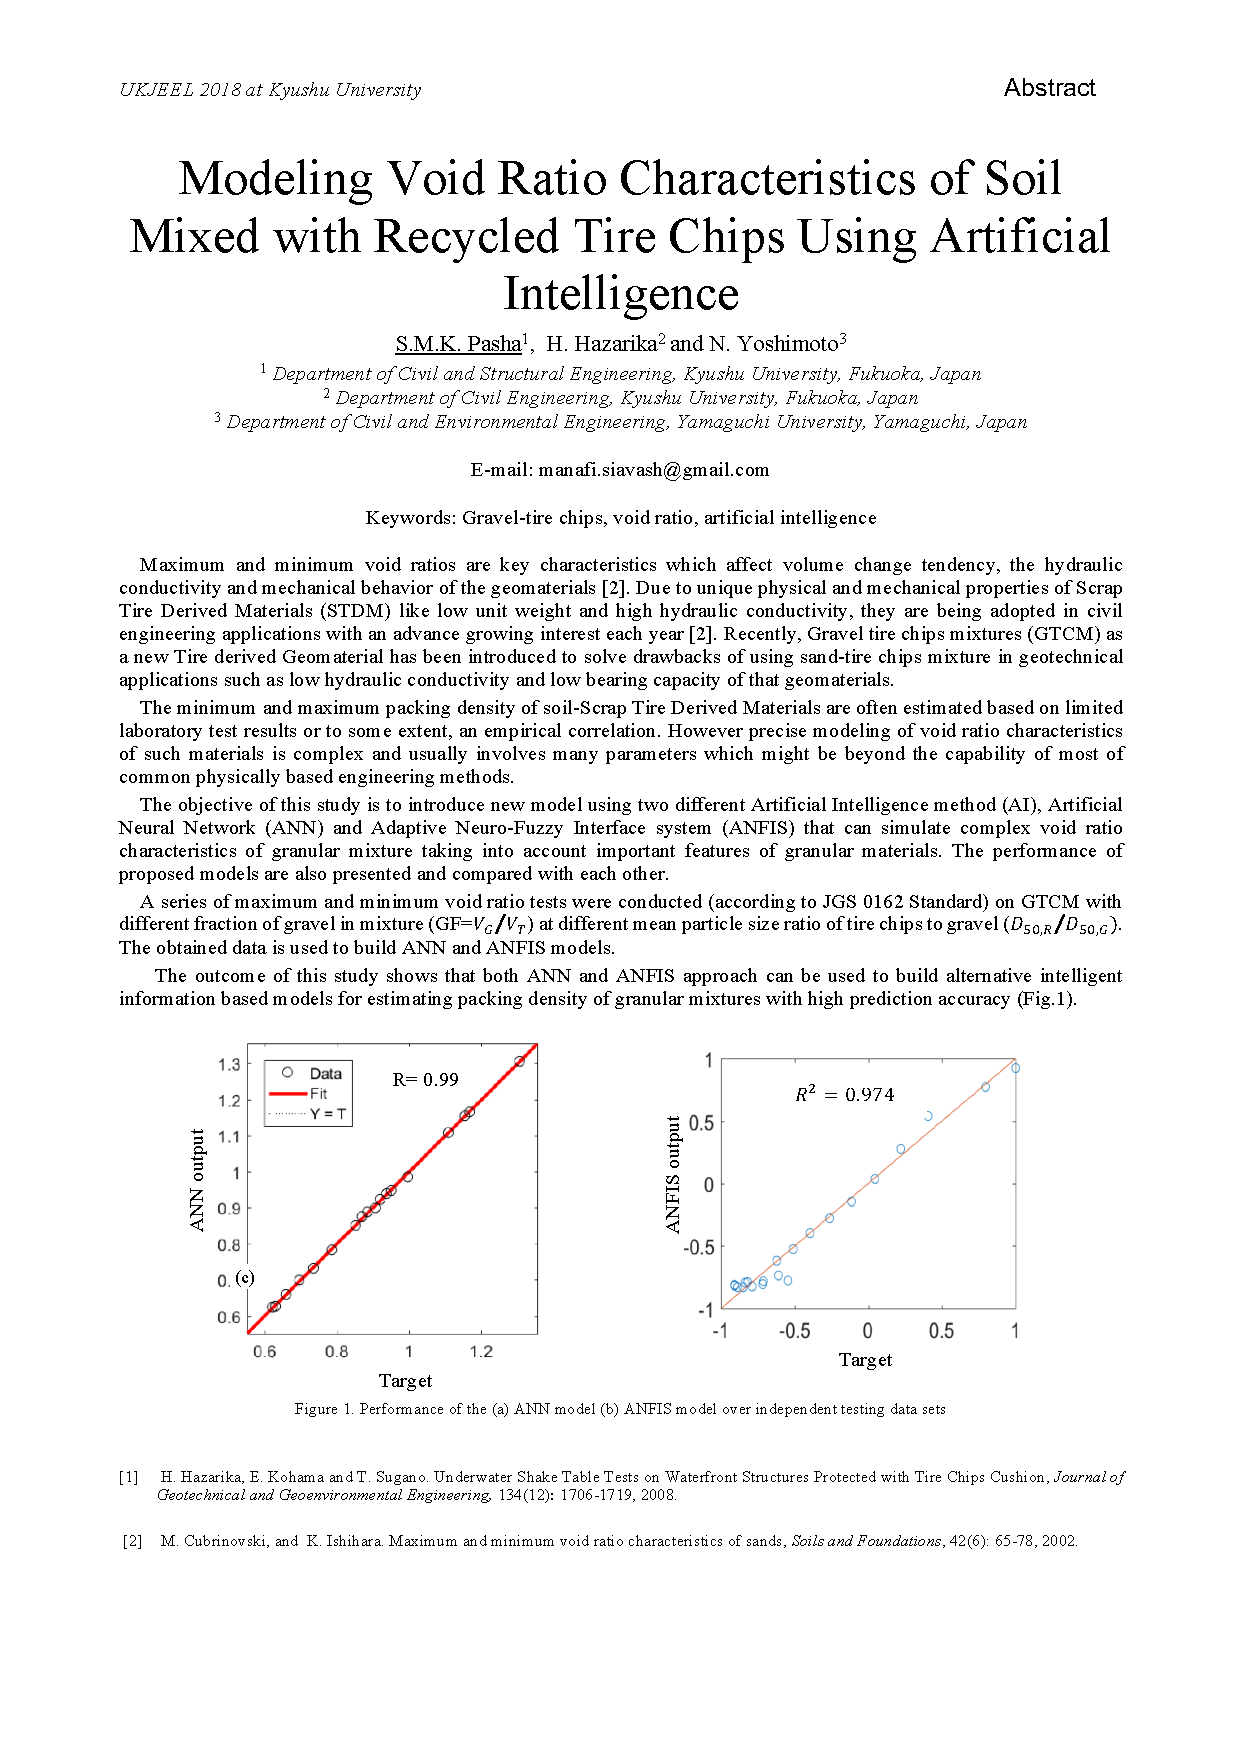
\includepdf[pagecommand={}]{abstracts/28-UKJEEL2018_Manafi-Hazarika-Yoshimoto.pdf}

 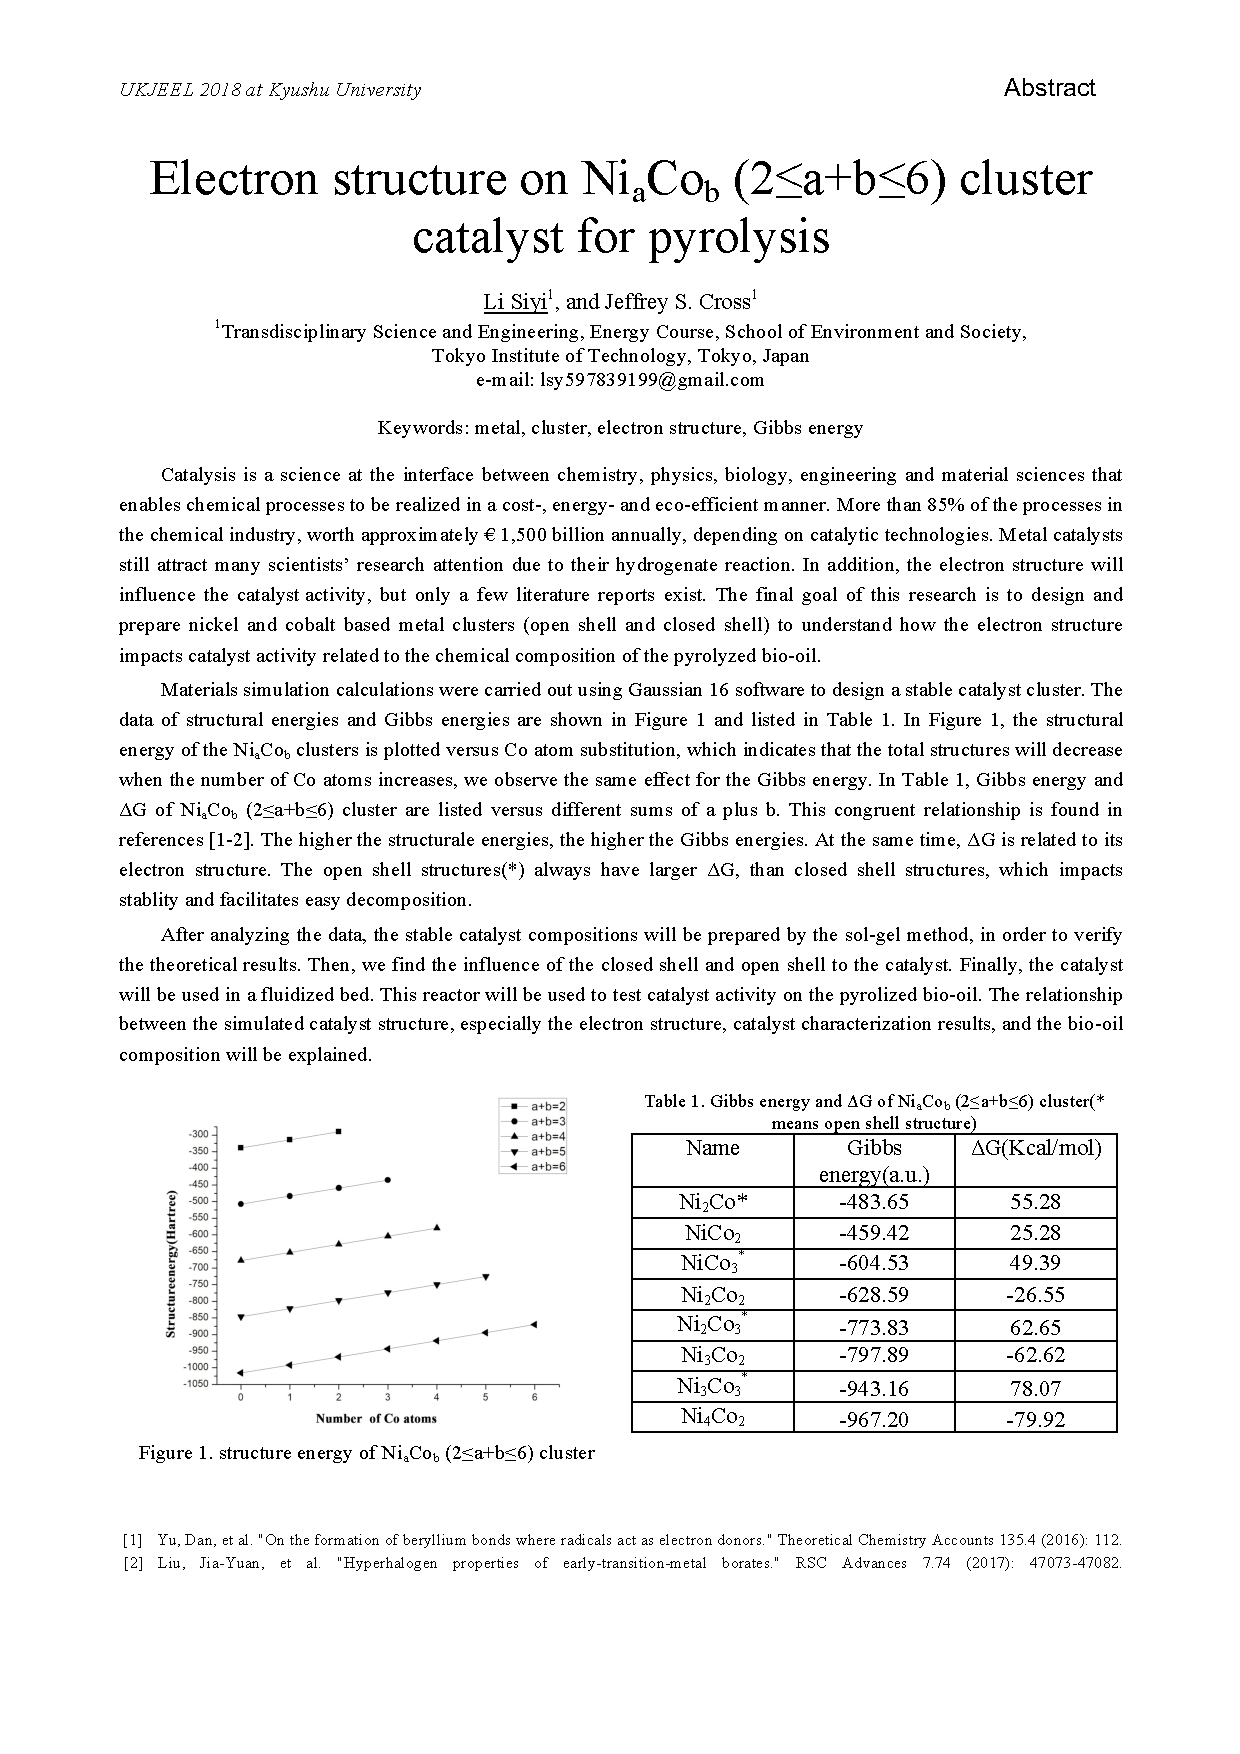
\includepdf[pagecommand={}]{abstracts/01-UKJEEL_Li-Siyi.pdf}

 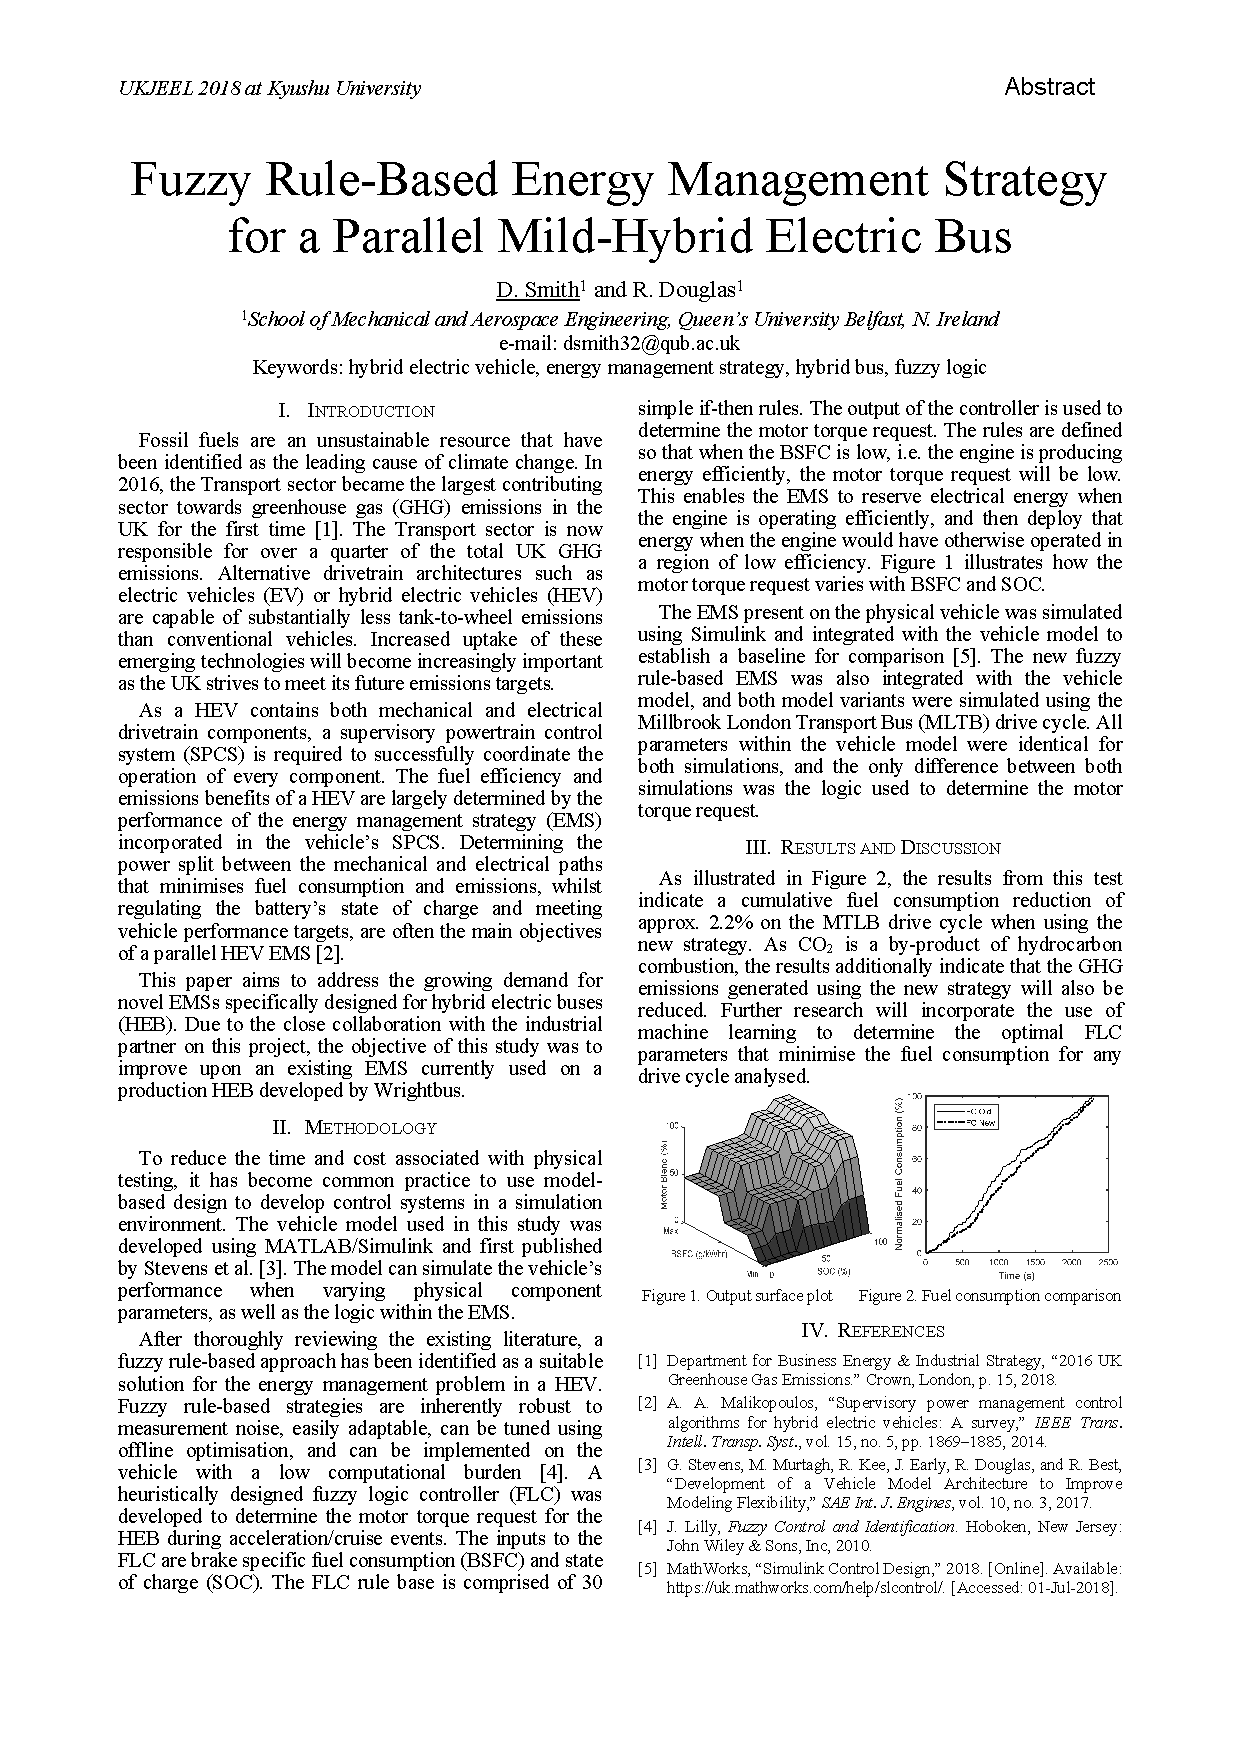
\includepdf[pagecommand={}]{abstracts/05-UKJEEL_Smith-Dan.pdf}

 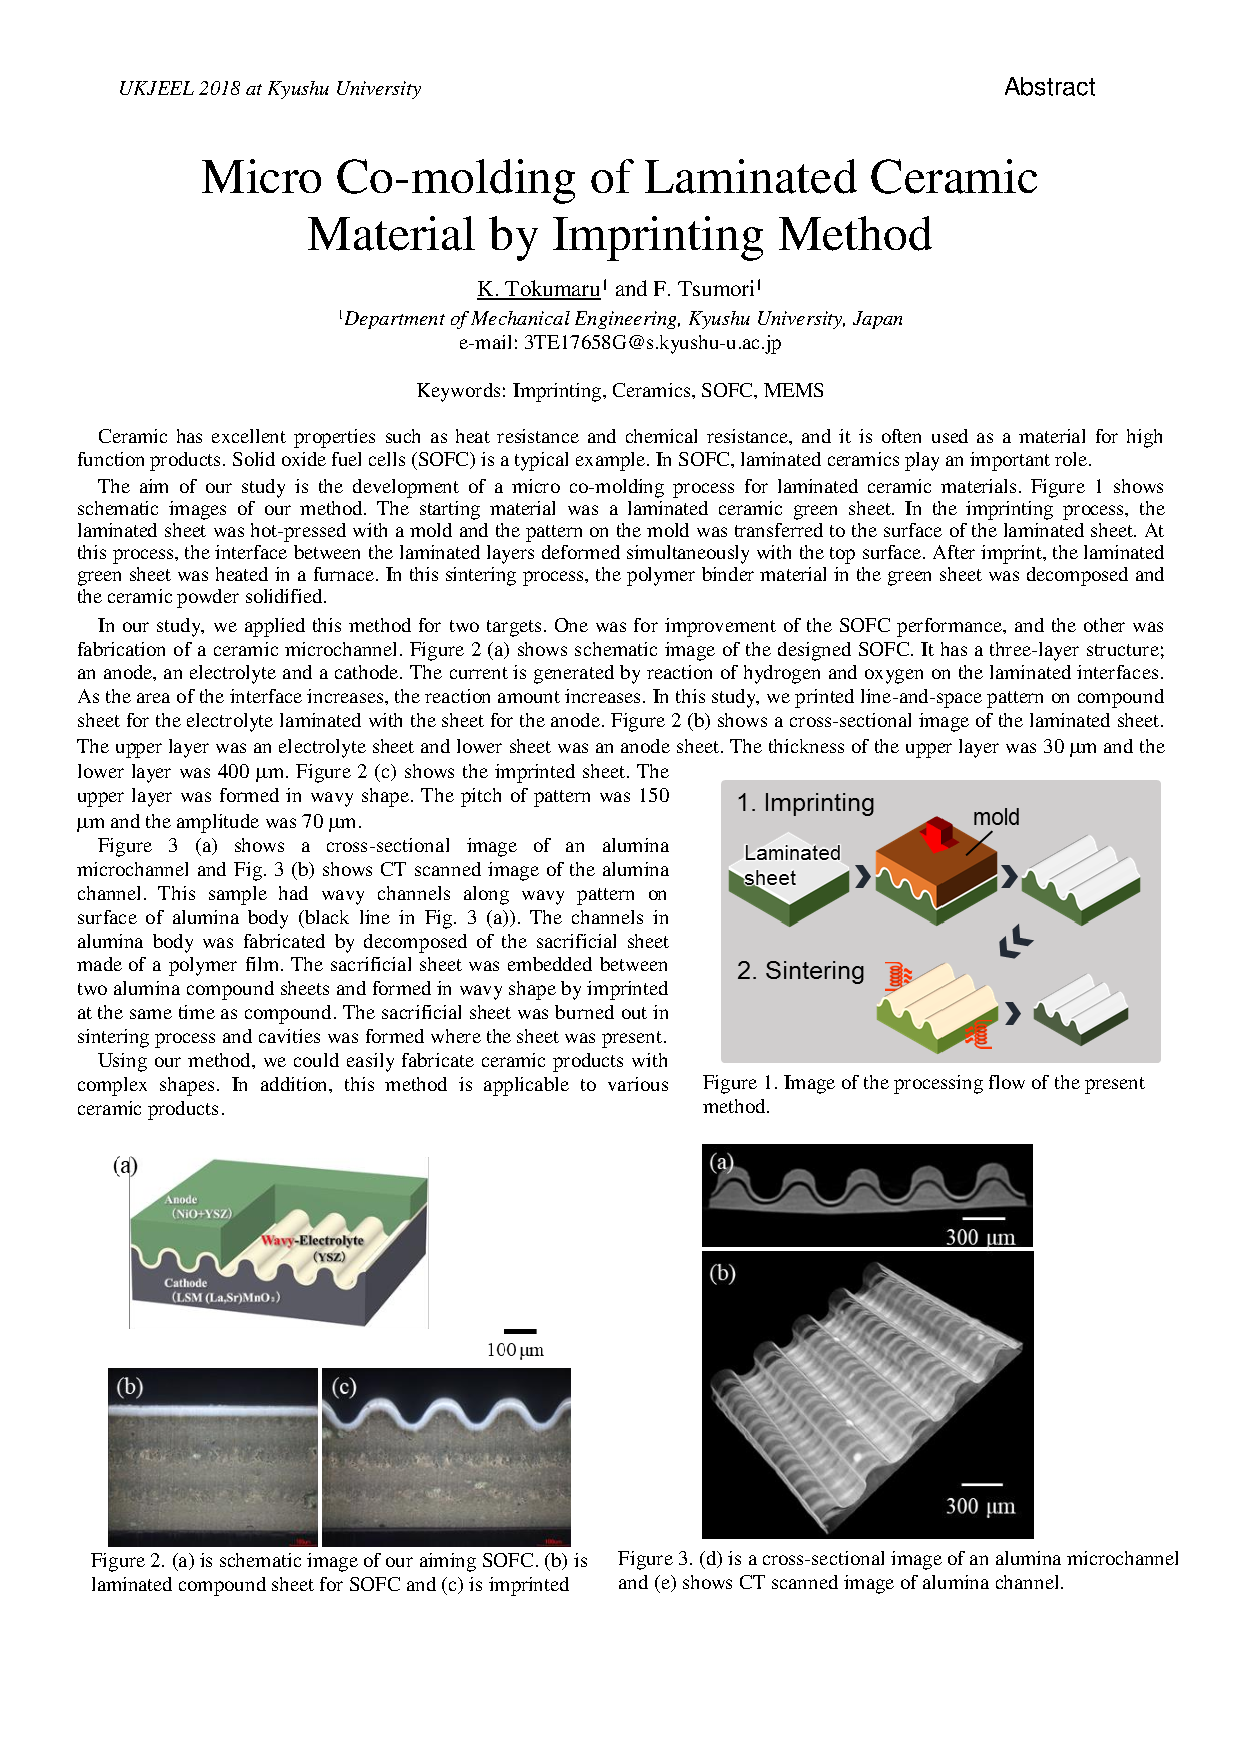
\includepdf[pagecommand={}]{abstracts/18-UKJEEL_Kazuki-Tokumaru.pdf}

 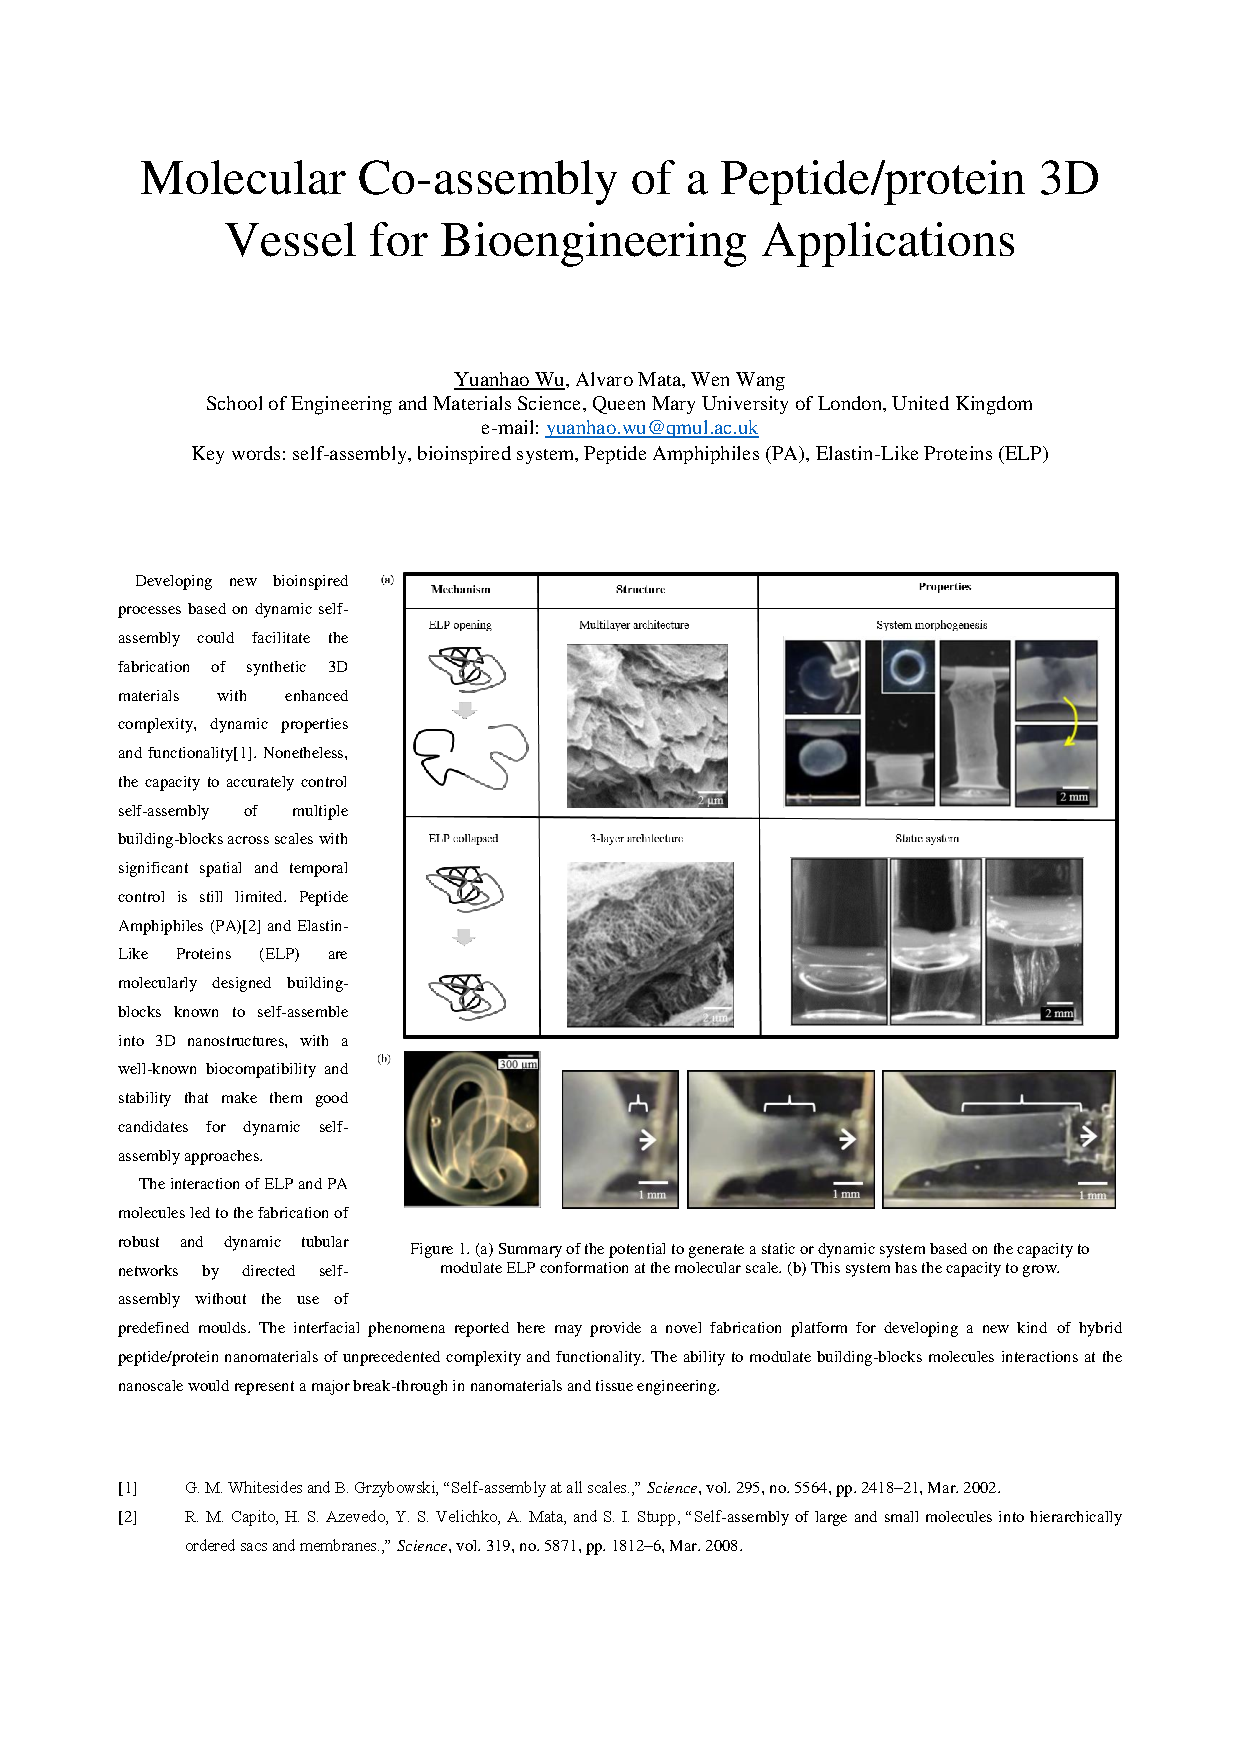
\includepdf[pagecommand={}]{abstracts/19-UKJEEL_Yuanhao-WU.pdf}

 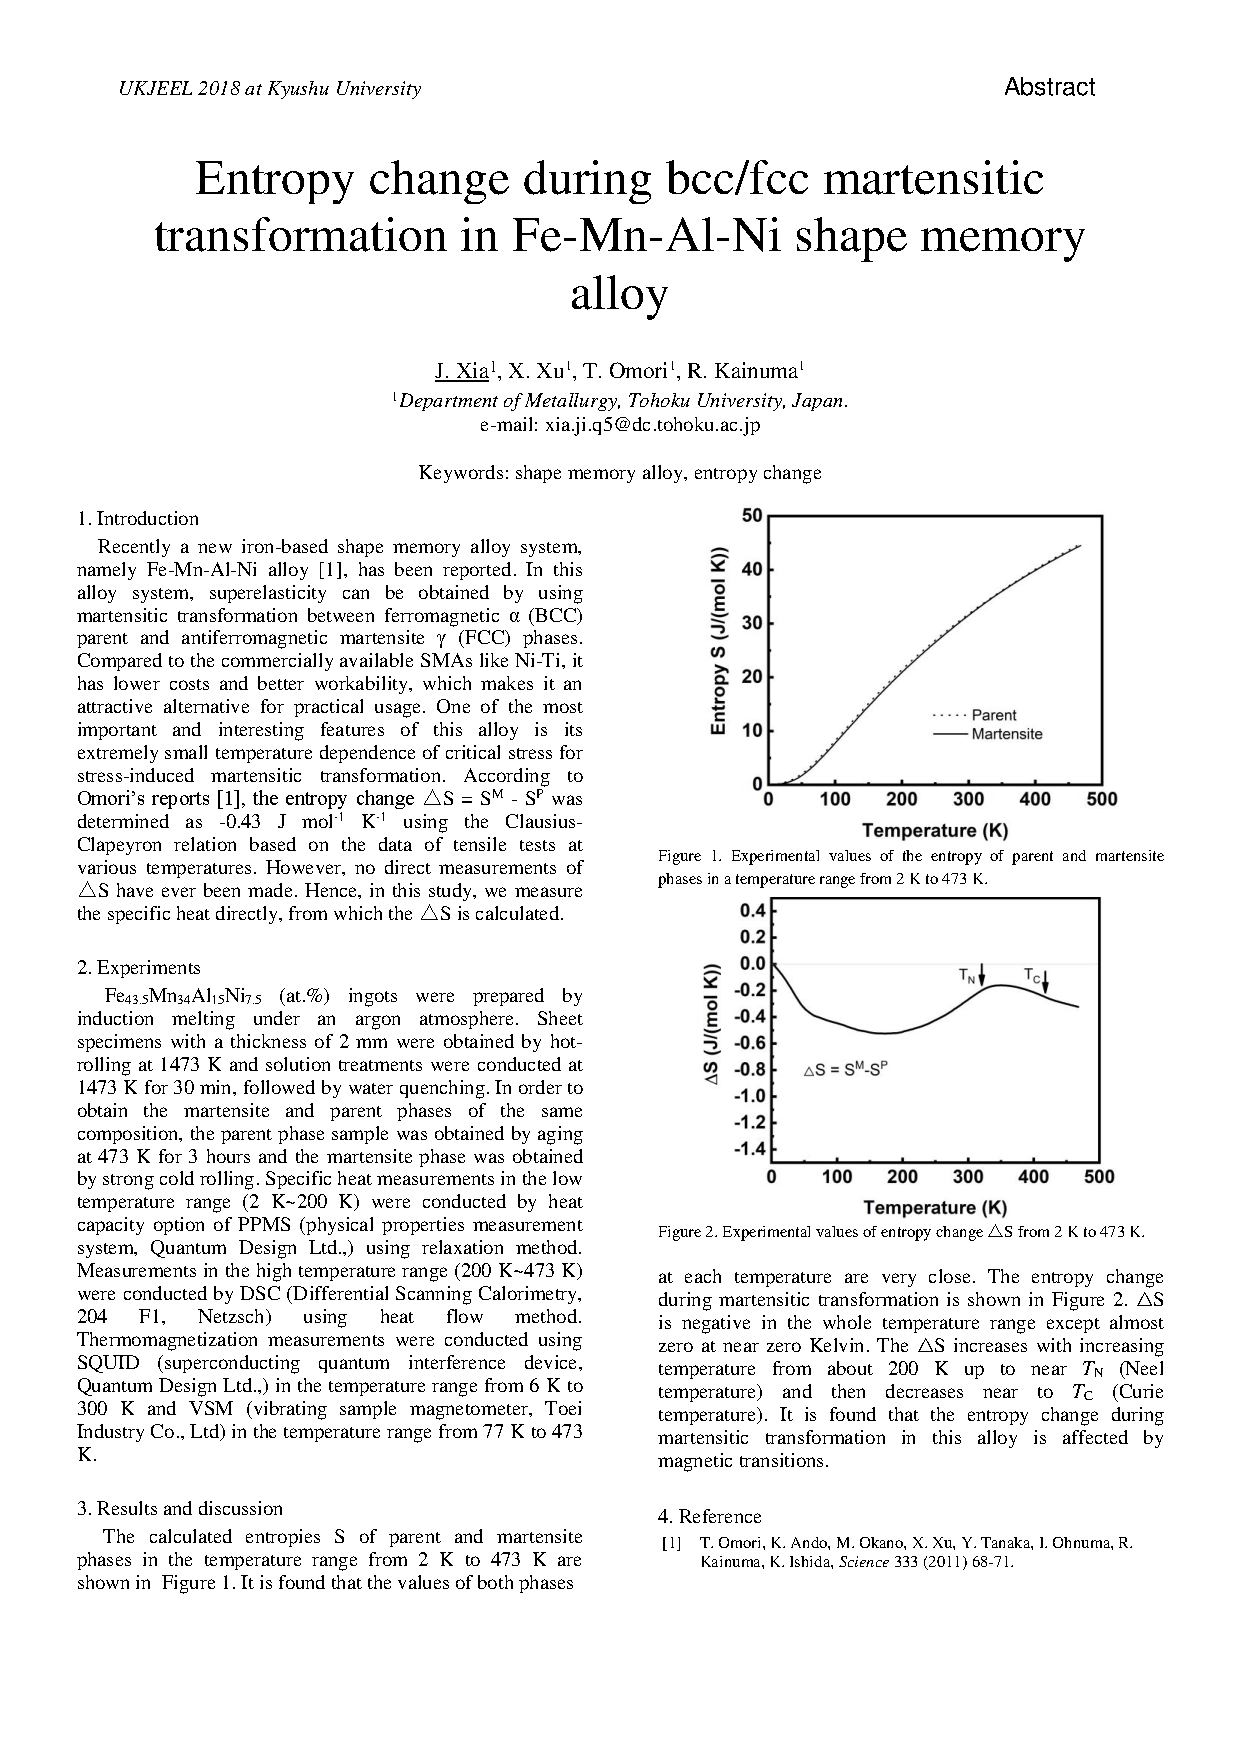
\includepdf[pagecommand={}]{abstracts/12-UKJEEL2018_XiaJi.pdf}

 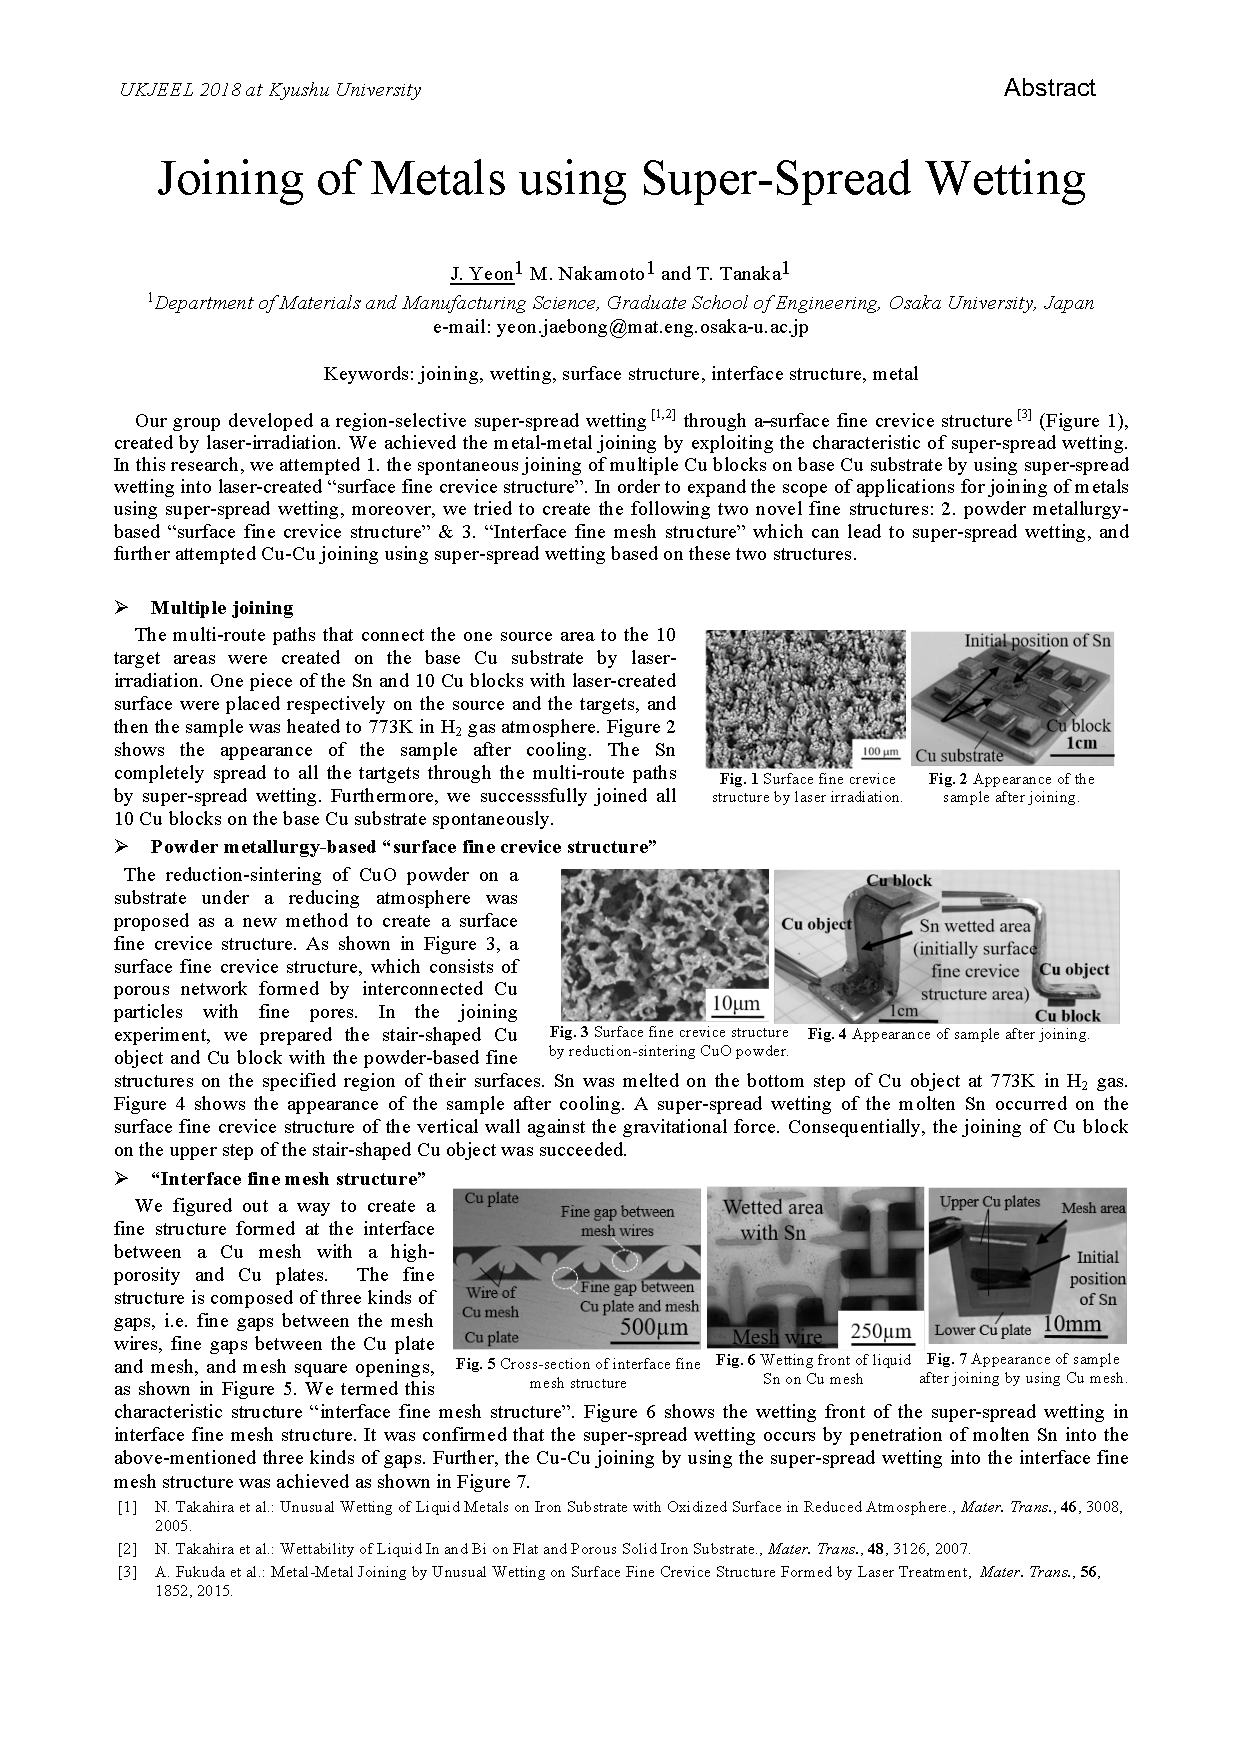
\includepdf[pagecommand={}]{abstracts/16-UKJEEL2018_Yeon.pdf}

 



 % Title page + PDF inserts of abstracts
\backmatter %[DW] Can only be used with 'book'
\section{Maps}
[Insert map of Nishijin plaza layout and local area map here.]


\end{document}

